\documentclass[aspectratio=169,10pt]{beamer}

\usepackage[T1]{fontenc}
\usepackage[utf8]{inputenc}
\usepackage{microtype}
\usepackage{tgheros}
\usepackage[scaled=0.92]{inconsolata}
\renewcommand{\familydefault}{\sfdefault}
\usepackage{amsmath}
\usepackage{amssymb}
\usepackage{array}
\usepackage{booktabs}
\usepackage{graphicx}
\usepackage{multirow}
\usepackage{ragged2e}
\usepackage{tabularx}
\usepackage{tikz}
\usepackage[most]{tcolorbox}
\usepackage{pifont}
\usetikzlibrary{calc,positioning}

\definecolor{header}{HTML}{123B4A}
\definecolor{headerlight}{HTML}{D7E7EC}
\definecolor{accent}{HTML}{D98E32}
\definecolor{ink}{HTML}{222222}
\definecolor{muted}{HTML}{5A6770}
\definecolor{softgray}{HTML}{F3F5F6}
\definecolor{grayborder}{HTML}{D4D8DB}
\definecolor{goodgreen}{HTML}{2F7D4A}
\definecolor{warnred}{HTML}{9A3B2D}
\definecolor{bluehint}{HTML}{EDF4F8}

\newcommand{\decktextmargin}{0.62cm}
\newcommand{\frametitleleftinset}{\decktextmargin}

\setbeamersize{text margin left=\decktextmargin, text margin right=\decktextmargin}
\setbeamertemplate{navigation symbols}{}
\setbeamertemplate{headline}{}
\setbeamercolor{normal text}{fg=ink,bg=white}
\setbeamercolor{structure}{fg=header}
\setbeamercolor{frametitle}{fg=white,bg=header}
\setbeamercolor{page number in head/foot}{fg=muted,bg=white}
\setbeamercolor{block title}{fg=header,bg=softgray}
\setbeamercolor{block body}{fg=ink,bg=softgray}
\setbeamercolor{itemize item}{fg=accent}
\setbeamercolor{itemize subitem}{fg=accent}

\setbeamerfont{frametitle}{size=\normalsize,series=\bfseries}
\setbeamerfont{framesubtitle}{size=\small}
\setbeamerfont{title}{size=\Huge,series=\bfseries}
\setbeamerfont{subtitle}{size=\Large}
\setbeamerfont{page number in head/foot}{size=\footnotesize,series=\bfseries}
\setbeamerfont{block title}{size=\normalsize,series=\bfseries}
\setbeamerfont{block body}{size=\small}

\setbeamertemplate{itemize item}{\color{accent}\scriptsize\ding{110}}
\setbeamertemplate{itemize subitem}{\color{accent}\tiny\ding{118}}

\makeatletter
\newcommand{\pagenumberrightinset}{0.19cm}
\newcommand{\pagenumberbottominset}{0.20cm}
\newcommand{\deckpagenumbers}{{\ttfamily\usebeamerfont{page number in head/foot}\insertframenumber\kern0.1em/\kern0.1em\inserttotalframenumber}}
\newcommand{\fullbleedbox}[2]{%
  \makebox[0pt][l]{%
    \hspace*{-\decktextmargin}%
    \begin{beamercolorbox}[wd=\paperwidth,ht=#1,dp=0pt,#2]{frametitle}%
    \end{beamercolorbox}%
  }%
  \vspace*{#1}%
}
\newcommand{\deckpagenumberoverlay}{%
  \begin{tikzpicture}[remember picture,overlay]
    \node[
      anchor=south east,
      inner sep=0pt,
      text=muted,
      font=\ttfamily\footnotesize\bfseries
    ] at ([xshift=-\pagenumberrightinset,yshift=\pagenumberbottominset]current page.south east) {\deckpagenumbers};
  \end{tikzpicture}%
}
\let\plainpagenumberoverlay\deckpagenumberoverlay
\newcommand{\plainheaderband}[1]{%
  \begin{tikzpicture}[remember picture,overlay]
    \path[fill=header] (current page.north west) rectangle ([yshift=-#1]current page.north east);
  \end{tikzpicture}%
}
\setbeamertemplate{frametitle}{%
  \nointerlineskip%
  \begin{beamercolorbox}[wd=\paperwidth,ht=0.74cm,dp=0cm,sep=0pt]{frametitle}
    \vbox to 0.74cm{%
      \vfil
      \hspace*{\frametitleleftinset}%
      \parbox[t]{\textwidth}{%
        {\usebeamerfont{frametitle}\strut\insertframetitle\par}%
        \ifx\insertframesubtitle\@empty\else%
          {\usebeamerfont{framesubtitle}\color{headerlight}\insertframesubtitle\par}%
        \fi
      }%
      \vfil
    }%
  \end{beamercolorbox}%
}
\makeatother

\setbeamertemplate{footline}{%
  \leavevmode%
  \hbox{%
    \begin{beamercolorbox}[wd=\paperwidth,ht=2.25ex,dp=1.1ex]{page number in head/foot}%
    \end{beamercolorbox}%
  }%
  \deckpagenumberoverlay%
}

\renewcommand{\arraystretch}{1.18}
\newcolumntype{Y}{>{\RaggedRight\arraybackslash}X}
\newcolumntype{M}[1]{>{\centering\arraybackslash}m{#1}}

\newcommand{\code}[1]{\texttt{#1}}
\newcommand{\term}[1]{{\color{header}\textbf{#1}}}
\newcommand{\miniheading}[1]{\vspace{0.1cm}{\color{header}\bfseries #1}\par\vspace{0.06cm}}
\newcommand{\sourceline}[1]{}
\newcommand{\datasourceline}[1]{\vspace{0.14em}{\raggedright\scriptsize\color{muted}\textbf{Source:} #1\par}}
\newenvironment{callout}
  {\begin{tcolorbox}[colback=accent!7!white,colframe=accent,boxrule=0.5pt,arc=2mm,left=1.5mm,right=1.5mm,top=1mm,bottom=1mm]\small}
  {\end{tcolorbox}}

\tcbset{
  deckbox/.style={
    enhanced,
    boxrule=0.35pt,
    arc=2mm,
    colback=softgray,
    colframe=grayborder,
    left=1.5mm,
    right=1.5mm,
    top=1.1mm,
    bottom=1.1mm,
    boxsep=0.5mm
  }
}

\newenvironment{softbox}
  {\begin{tcolorbox}[deckbox]}
  {\end{tcolorbox}}

\newenvironment{pseudobox}
  {\begin{tcolorbox}[deckbox,colback=black!2!white]\ttfamily\small}
  {\end{tcolorbox}}

\newcommand{\MetricTile}[2]{%
  \begin{tcolorbox}[deckbox,colback=bluehint,title=\textbf{#1},fonttitle=\small\bfseries,coltitle=header]
  \small #2
  \end{tcolorbox}
}

\newcommand{\SectionDivider}[3]{%
  \begin{frame}[plain]
    \plainheaderband{0.78cm}
    \begin{tikzpicture}[remember picture,overlay]
      \node[
        anchor=center,
        align=center,
        text=ink,
        text width=0.86\paperwidth,
        font=\bfseries\fontsize{19}{23}\selectfont
      ] at ([yshift=0.18cm]current page.center) {#1};
      \fill[softgray] ([xshift=0.62cm,yshift=1.78cm]current page.south west) rectangle ([xshift=-0.62cm,yshift=1.94cm]current page.south east);
      \pgfmathsetmacro{\progressfraction}{(#2)/(#3)}
      \path let \p1 = ([xshift=0.62cm,yshift=1.78cm]current page.south west), \p2 = ([xshift=-0.62cm,yshift=1.94cm]current page.south east) in
        [fill=accent] (\p1) rectangle ({\x1 + \progressfraction*(\x2-\x1)}, \y2);
    \end{tikzpicture}
    \plainpagenumberoverlay
  \end{frame}
}

\newcommand{\AppendixDivider}[1]{%
  \begin{frame}[plain]
    \plainheaderband{0.78cm}
    \begin{tikzpicture}[remember picture,overlay]
      \node[
        anchor=center,
        align=center,
        text=ink,
        text width=0.88\paperwidth,
        font=\bfseries\fontsize{17}{21}\selectfont
      ] at ([yshift=0.18cm]current page.center) {#1};
      \fill[accent] ([xshift=0.62cm,yshift=1.78cm]current page.south west) rectangle ([xshift=-0.62cm,yshift=1.94cm]current page.south east);
    \end{tikzpicture}
    \plainpagenumberoverlay
  \end{frame}
}

\newcommand{\TitleFrame}[4]{%
  \begin{frame}[plain]
    \begin{tikzpicture}[remember picture,overlay]
      \path[fill=header] (current page.north west) rectangle ([yshift=-1.26cm]current page.north east);
      \path[fill=accent] ([yshift=-1.26cm]current page.north west) rectangle ([yshift=-1.38cm]current page.north east);
      \node[
        anchor=west,
        text=white,
        font=\bfseries\fontsize{19}{23}\selectfont
      ] at ([xshift=0.62cm,yshift=-0.70cm]current page.north west) {#1};
      \node[
        anchor=north west,
        align=left,
        text=header,
        text width=0.90\paperwidth,
        font=\bfseries\Large
      ] at ([xshift=0.62cm,yshift=-1.62cm]current page.north west) {#2};
    \end{tikzpicture}
    \vspace*{3.18cm}
    \begin{center}
      \begin{minipage}{0.88\textwidth}
        \begin{softbox}
          \small #3
        \end{softbox}
      \end{minipage}
    \end{center}
    \vspace{0.04cm}
    {\centering\small\color{muted}#4\par}
    \plainpagenumberoverlay
  \end{frame}
}

\graphicspath{{assets/}}

\begin{document}

\TitleFrame
  {PETSc Rewrite of Slope Stability}
  {From the legacy MATLAB workflow to the current PETSc runtime}
  {
    \begin{itemize}
      \item Translate the original MATLAB mental model into the current executable PETSc/Python path.
      \item Show where parallel ownership, PMG, unified runners, unified meshes, and unified visualisation changed the design.
    \end{itemize}
  }
  {Repository-local material only. Snapshot date: April 13, 2026.}

\begin{frame}{Agenda}
\small
\begin{softbox}
\begin{enumerate}
  \item MATLAB baseline
  \item What changed structurally
  \item What is new and reusable
  \item How to add a new benchmark
  \item Unified visualisation
  \item Unified meshes
  \item Speed comparison
  \item Where to edit the code and close
\end{enumerate}
\end{softbox}
\end{frame}

\begin{frame}{Repository Sources Used Here}
\small
\begin{columns}[T,totalwidth=\textwidth]
\begin{column}{0.32\textwidth}
\MetricTile{Legacy MATLAB Entry Points}{
\code{3D\_hetero\_SSR.m}\\
\code{+CONTINUATION/*}\\
\code{+NEWTON/*}\\
\code{+CONSTITUTIVE\_PROBLEM/*}\\
\code{+MESH/*}\\
\code{+VIZ/*}
}
\end{column}
\begin{column}{0.32\textwidth}
\MetricTile{PETSc Runtime Entry Points}{
\code{README.md}\\
\code{run\_config.py}\\
\code{run\_case\_from\_config.py}\\
\code{execution/asset\_case/runner.py}
}
\end{column}
\begin{column}{0.32\textwidth}
\MetricTile{Local Docs And Studies}{
\code{petsc\_matlab\_map}\\
\code{config-scheme-3d.md}\\
\code{config-case-matrix.md}\\
\code{performance\_comparison}
}
\end{column}
\end{columns}
\vspace{0.22cm}
\begin{softbox}
\miniheading{How the material is used}
Architecture statements in this presentation are anchored on the default 3D heterogeneous SSR \code{P4}/PMG benchmark, because it exercises the current mainline path. Runtime comparisons later in the presentation come from the committed \code{P2} study, so architecture and performance evidence stay separate.
\end{softbox}
\end{frame}

\SectionDivider{MATLAB Baseline}{1}{8}

\begin{frame}{The Legacy Execution Model Is Script-Centric}
\small
\begin{columns}[T,totalwidth=\textwidth]
\begin{column}{0.56\textwidth}
\begin{softbox}
\begin{itemize}
  \item One benchmark usually equals one top-level script.
  \item \code{slope\_stability\_3D\_hetero\_SSR.m} declares the case, chooses the solver, launches continuation, and plots the results.
  \item The numerical kernels are modular, but orchestration remains case-local rather than config-driven.
  \item The workflow is learned by reading the script from top to bottom.
\end{itemize}
\end{softbox}
\end{column}
\begin{column}{0.40\textwidth}
\begin{pseudobox}
start\\
$\rightarrow$ quadrature\\
$\rightarrow$ local basis\\
$\rightarrow$ mesh load\\
$\rightarrow$ material expansion + labels\\
$\rightarrow$ \code{K\_elast}, \code{B}, \code{f\_V}\\
$\rightarrow$ constitutive object\\
$\rightarrow$ SSR continuation\\
$\rightarrow$ MATLAB figures
\end{pseudobox}
\end{column}
\end{columns}
\sourceline{\code{slope\_stability\_matlab/slope\_stability\_3D\_hetero\_SSR.m}}
\end{frame}

\begin{frame}{MATLAB Package Map}
\small
\begin{tabularx}{\textwidth}{p{0.24\textwidth}p{0.33\textwidth}Y}
\toprule
\textbf{Package} & \textbf{Role} & \textbf{Typical content} \\
\midrule
\code{+ASSEMBLY} & FE preprocessing & Quadrature, local basis, elastic stiffness, volume forces, material expansion \\
\code{+CONTINUATION} & Outer branch tracking & Direct SSR, indirect SSR, LL, init phase, omega stepping \\
\code{+NEWTON} & Nonlinear solve core & Damped Newton, indirect SSR Newton, LL Newton \\
\code{+CONSTITUTIVE\_PROBLEM} & Stress and tangent model & Davis reduction, stress evaluation, tangent assembly, potential \\
\code{+LINEAR\_SOLVERS} & Linear solver factory & Direct, AGMG, ICHOL, HYPRE BoomerAMG, DFGMRES, collectors \\
\code{+MESH}, \code{+VIZ}, \code{+SEEPAGE} & Domain-specific helpers & Case loaders, plotting, seepage preprocessing and flow solve \\
\bottomrule
\end{tabularx}
\sourceline{\code{slope\_stability\_matlab/+ASSEMBLY}; \code{slope\_stability\_matlab/+CONTINUATION}; \code{slope\_stability\_matlab/+VIZ}}
\end{frame}

\begin{frame}{MATLAB Continuation And Newton Paths}
\small
\begin{columns}[T,totalwidth=\textwidth]
\begin{column}{0.49\textwidth}
\begin{softbox}
\miniheading{Common benchmark solve flow}
\begin{itemize}
  \item The benchmark script selects the analysis, continuation path, solver handle, and stopping settings.
  \item The nonlinear path then branches into direct SSR, indirect SSR, or indirect LL continuation.
  \item Each continuation path calls a matching Newton kernel and damping path.
  \item Accepted steps extend the history arrays; rejected steps shrink and retry.
\end{itemize}
\end{softbox}
\end{column}
\begin{column}{0.49\textwidth}
\begin{softbox}
\miniheading{Main nonlinear branches}
\begin{tabularx}{\linewidth}{p{0.27\linewidth}Y}
\textbf{Direct SSR} & \code{SSR\_direct\_continuation.m} $\rightarrow$ \code{NEWTON.newton} \\
\textbf{Indirect SSR} & \code{SSR\_indirect\_continuation.m} $\rightarrow$ \code{NEWTON.newton\_ind\_SSR} \\
\textbf{Indirect LL} & \code{LL\_indirect\_continuation.m} $\rightarrow$ \code{NEWTON.newton\_ind\_LL} \\
\end{tabularx}
\end{softbox}
\end{column}
\end{columns}
\sourceline{\code{slope\_stability\_matlab/+CONTINUATION/SSR\_direct\_continuation.m}; \code{slope\_stability\_matlab/+CONTINUATION/SSR\_indirect\_continuation.m}; \code{slope\_stability\_matlab/+CONTINUATION/LL\_indirect\_continuation.m}}
\end{frame}

\begin{frame}{MATLAB Constitutive Object Is Already A Central Kernel}
\small
\begin{columns}[T,totalwidth=\textwidth]
\begin{column}{0.52\textwidth}
\begin{softbox}
\miniheading{Constitutive kernel role}
\begin{itemize}
  \item \code{CONSTITUTIVE} centralises Davis reduction, stress evaluation, tangent evaluation, residual assembly, and timing collectors.
  \item The object owns the integration-point material fields and mediates calls into the lower-level constitutive functions.
  \item This is already the closest MATLAB analogue of the PETSc constitutive operator.
\end{itemize}
\end{softbox}
\end{column}
\begin{column}{0.44\textwidth}
\begin{pseudobox}
script / continuation\\
$\rightarrow$ constitutive object\\
$\rightarrow$ reduction + stress\\
$\rightarrow$ tangent + residual\\
$\rightarrow$ Newton / continuation history
\end{pseudobox}
\vspace{0.16cm}
\begin{callout}
The constitutive wrapper already exists in MATLAB. The rewrite changes the ownership and assembly model around it.
\end{callout}
\end{column}
\end{columns}
\sourceline{\code{slope\_stability\_matlab/+CONSTITUTIVE\_PROBLEM/CONSTITUTIVE.m}; \code{slope\_stability\_matlab/+CONSTITUTIVE\_PROBLEM/constitutive\_problem\_3D.m}}
\end{frame}
\begin{frame}{Mesh, Materials, And Dirichlet Labels In MATLAB Are Closely Coupled}
\small
\begin{tabularx}{\textwidth}{p{0.28\textwidth}p{0.30\textwidth}Y}
\toprule
\textbf{MATLAB path} & \textbf{What it assumes} & \textbf{Consequence} \\
\midrule
\code{load\_mesh\_P2.m} & Quadratic tetrahedral HDF5 input & Benchmark meshes and FE degree are tied together \\
\code{load\_mesh\_gmsh\_waterlevels.m} & Case-specific Gmsh seepage conventions & Loader logic lives with the case family \\
\code{midpoints\_P2.m}, \code{midpoints\_P4.m} & Degree-specific node generation & Higher order support grows through dedicated utilities \\
\code{Q} mask from face labels & BC labels are interpreted in the loader path & Free-DOF extraction depends on the loaded mesh convention \\
\code{material\_identif} expansion & Material ids are resolved during loading & Material heterogeneity is coupled to the same loader decisions \\
\bottomrule
\end{tabularx}
\vspace{0.18cm}
\begin{callout}
This is one of the biggest conceptual changes in the rewrite: the PETSc side moves toward \term{canonical mesh family storage} plus \term{solver-side degree selection}, instead of one file format per numerical path.
\end{callout}
\sourceline{\code{slope\_stability\_matlab/+MESH/load\_mesh\_P2.m}; \code{slope\_stability\_matlab/+MESH/load\_mesh\_gmsh\_waterlevels.m}}
\end{frame}

\begin{frame}{MATLAB Visualisation Still Lives Inside The Case Script}
\small
\begin{columns}[T,totalwidth=\textwidth]
\begin{column}{0.56\textwidth}
\begin{softbox}
\miniheading{What the MATLAB flow still does well}
\begin{itemize}
  \item The benchmark script can call \code{VIZ.*} immediately after the solve and inspect the same assembled state.
  \item That keeps the familiar 3D and slice figures close to the benchmark logic the original authors already know.
\end{itemize}
\end{softbox}
\begin{softbox}
\miniheading{What stays coupled}
\begin{tabularx}{\linewidth}{p{0.30\linewidth}Y}
\textbf{state} & live MATLAB workspace after the solve \\
\textbf{plots} & benchmark-local \code{VIZ.*} calls and figure setup \\
\textbf{reuse} & copy-and-adapt workflow between benchmark families \\
\end{tabularx}
\end{softbox}
\end{column}
\begin{column}{0.40\textwidth}
\begin{pseudobox}
start\\
$\rightarrow$ solve benchmark\\
\(\rightarrow\) call \code{VIZ.*}\\
\(\rightarrow\) inspect figure state\\
\(\rightarrow\) export figure manually\\
\(\rightarrow\) repeat per case family
\end{pseudobox}
\vspace{0.18cm}
\begin{callout}
The figure family stays comparable. The production path changes: case-local plotting code and live interpreter state are replaced by shared exports and notebook reconstruction.
\end{callout}
\end{column}
\end{columns}
\end{frame}

\SectionDivider{What Changed Structurally}{2}{8}

\begin{frame}{What Stays Familiar, What Changes}
\small
\begin{columns}[T,totalwidth=\textwidth]
\begin{column}{0.48\textwidth}
\MetricTile{Familiar problem structure}{
\begin{itemize}
  \item SSR and LL as the benchmark families people already recognize
  \item Newton plus step accept-or-shrink logic
  \item Davis reduction and the constitutive kernel as the physical core
  \item continuation outputs such as \(\lambda\), \(\omega\), and \(u_{\max}\)
\end{itemize}
}
\end{column}
\begin{column}{0.48\textwidth}
\MetricTile{Changed runtime structure}{
\begin{itemize}
  \item top-level script orchestration
  \item one global sparse rebuild per Newton step
  \item one solver-handle-only view of the linear solve
  \item workspace-local outputs and plotting state
\end{itemize}
}
\end{column}
\end{columns}
\vspace{0.16cm}
\begin{callout}
The mathematics is still familiar. The execution packaging, ownership model, and reusable interfaces are what changed.
\end{callout}
\end{frame}

\begin{frame}{Responsibility Map: MATLAB Driver To PETSc Modules}
\small
\begin{tabularx}{\textwidth}{p{0.25\textwidth}p{0.26\textwidth}Y}
\toprule
\textbf{Role} & \textbf{MATLAB location} & \textbf{PETSc location} \\
\midrule
Case declaration & Top of the benchmark script & \code{case.toml} + \code{run\_config.py} \\
Runner dispatch & Implicit in the script name & \code{run\_case\_from\_config.py} \\
Mesh and material preprocessing & Script body + \code{+MESH}/\code{+ASSEMBLY} & \code{mesh/*} + \code{fem/*} + runner setup \\
Constitutive handle construction & \code{CONSTITUTIVE.m} & \code{problem.py:ConstitutiveOperator} \\
Continuation launch & \code{SSR\_indirect\_continuation.m} & \code{continuation/indirect.py} \\
Linear solver factory & \code{set\_linear\_solver.m} & \code{solver.py:SolverFactory} \\
\bottomrule
\end{tabularx}
\sourceline{\code{docs/petsc\_matlab\_map/chapters/mainline/01\_execution\_map.tex}}
\end{frame}

\begin{frame}{Architecture Anchor Benchmark}
\small
\begin{softbox}
\miniheading{Walk-through benchmark}
\begin{itemize}
  \item The checked-in 3D heterogeneous SSR default benchmark is the architecture anchor.
  \item It keeps the owned-row, overlap, \code{pmg\_shell}, and \code{P4} path in one place.
\end{itemize}
\vspace{0.04cm}
\begin{tabularx}{\linewidth}{@{}Y Y@{}}
\code{analysis = ssr} & \code{elem\_type = P4} \\
\code{node\_ordering = block\_metis} & \code{mpi\_distribute\_by\_nodes = true} \\
\code{constitutive\_mode = overlap} & \code{tangent\_kernel = rows} \\
\code{pc\_backend = pmg\_shell} & \\
\end{tabularx}
\end{softbox}
\vspace{0.16cm}
\begin{pseudobox}
start\\
$\rightarrow$ load config $\rightarrow$ resolve asset and route $\rightarrow$ build and reorder mesh\\
$\rightarrow$ build owned elastic rows $\rightarrow$ prepare owned tangent pattern\\
$\rightarrow$ create constitutive operator $\rightarrow$ build PETSc solver\\
$\rightarrow$ launch indirect SSR continuation
\end{pseudobox}
\end{frame}

\begin{frame}{Config Load And Runner Dispatch}
\small
\begin{columns}[T,totalwidth=\textwidth]
\begin{column}{0.54\textwidth}
\begin{softbox}
\miniheading{Config side}
\begin{itemize}
  \item \code{core/run\_config.py} loads TOML, validates \code{elem\_type}, analysis kind, and the asset-first public section shapes.
  \item The config object preserves the same high-level blocks MATLAB already used: problem, continuation, Newton, linear solver, and outputs.
  \item Materials, hydraulics, and boundary conditions are resolved from \code{meshes/<asset>/definition.py}, not local config rows.
\end{itemize}
\end{softbox}
\end{column}
\begin{column}{0.42\textwidth}
\begin{pseudobox}
cfg = load\_run\_case\_config(...)\\
asset = resolve\_problem\_asset(cfg)\\
route = select\_case\_route(cfg)\\
result = run\_case\_config(cfg)\\
write debug bundle\\
write history\\
write VTU
\end{pseudobox}
\end{column}
\end{columns}
\sourceline{\code{src/slope\_stability/core/run\_config.py}; \code{src/slope\_stability/cli/run\_case\_from\_config.py}}
\end{frame}

\begin{frame}{Assembly Policy And Node Ownership Are First-Class Decisions}
\small
\begin{columns}[T,totalwidth=\textwidth]
\begin{column}{0.50\textwidth}
\begin{softbox}
\miniheading{Policy inputs}
\begin{itemize}
  \item \code{solver\_type}
  \item \code{mpi\_distribute\_by\_nodes}
  \item \code{constitutive\_mode}
  \item \code{node\_ordering}
\end{itemize}
\miniheading{Default outcome}
\begin{itemize}
  \item owned tangent path enabled
  \item lightweight MPI elastic path enabled
  \item node numbering aligned to ownership through \code{block\_metis}
\end{itemize}
\end{softbox}
\end{column}
\begin{column}{0.46\textwidth}
\begin{callout}
\textbf{Why this matters}\\[0.12cm]
MATLAB kept one global sparse operator in one address space.\\[0.18cm]
The PETSc rewrite makes row ownership explicit early, because that ownership controls:
\begin{itemize}
  \item local element overlap
  \item constitutive work placement
  \item matrix assembly
  \item preconditioner construction
\end{itemize}
\end{callout}
\end{column}
\end{columns}
\sourceline{\code{src/slope\_stability/cli/assembly\_policy.py}; \code{docs/petsc\_matlab\_map/chapters/mainline/02\_mesh\_materials\_load.tex}}
\end{frame}

\begin{frame}{Owned Elastic Rows And A Fixed Tangent Pattern}
\small
\begin{columns}[T,totalwidth=\textwidth]
\begin{column}{0.48\textwidth}
\MetricTile{Prepared once}{
\begin{itemize}
  \item rank-owned node interval
  \item overlap elements for those rows
  \item local CSR matrix pattern
  \item elastic values on that pattern
  \item constrained diagonal positions
\end{itemize}
}
\end{column}
\begin{column}{0.48\textwidth}
\MetricTile{Refreshed every Newton step}{
\begin{itemize}
  \item constitutive state on overlap integration points
  \item internal force rows
  \item tangent values on the fixed CSR pattern
  \item regularised matrix blend \(K_r\)
\end{itemize}
}
\end{column}
\end{columns}
\vspace{0.18cm}
\begin{callout}
This is the deepest structural change relative to MATLAB: the rewrite no longer treats every Newton step as a fresh global sparse rebuild. The \term{structure} is prepared once; the \term{values} are refreshed in place.
\end{callout}
\sourceline{\code{src/slope\_stability/fem/distributed\_elastic.py}; \code{src/slope\_stability/fem/distributed\_tangent.py}}
\end{frame}

\begin{frame}{Overlap Constitutive Ownership And The Rows Kernel}
\small
\begin{columns}[T,totalwidth=\textwidth]
\begin{column}{0.49\textwidth}
\begin{softbox}
\miniheading{Overlap constitutive mode}
\begin{itemize}
  \item Each rank evaluates the constitutive model on the overlap integration points needed by its owned rows.
  \item The default path avoids a unique-owner recovery stage.
  \item The tangent kernel receives local overlap data directly.
\end{itemize}
\end{softbox}
\end{column}
\begin{column}{0.49\textwidth}
\begin{softbox}
\miniheading{Rows kernel}
\begin{itemize}
  \item The kernel walks the fixed owned CSR pattern row by row.
  \item Metadata such as \code{row\_slot\_ptr}, \code{slot\_elem}, \code{slot\_lrow}, and \code{slot\_pos} replace the old ``assemble element matrix, then scatter'' view.
  \item The bilinear form is unchanged; the dataflow is not.
\end{itemize}
\end{softbox}
\end{column}
\end{columns}
\sourceline{\code{docs/petsc\_matlab\_map/chapters/mainline/05\_tangent\_assembly.tex}; \code{src/slope\_stability/fem/distributed\_tangent.py}}
\end{frame}

\begin{frame}{What \code{pmg\_shell} Means On This Mainline}
\small
\begin{columns}[T,totalwidth=\textwidth]
\begin{column}{0.53\textwidth}
\begin{softbox}
\begin{itemize}
  \item The fine-grid operator is the reduced free-space regularized operator coming from the owned-row tangent path.
  \item The outer Krylov family is still the PETSc-wrapped MATLAB-style deflated FGMRES interface.
  \item The actual preconditioner is a custom shell V-cycle, not the built-in PETSc \code{PCMG} path.
  \item The hierarchy metadata enters through \code{pmg\_hierarchy} and stays aligned with the same reordered free-space numbering as the solve operator.
\end{itemize}
\end{softbox}
\end{column}
\begin{column}{0.43\textwidth}
\begin{tabularx}{\linewidth}{p{0.32\linewidth}Y}
\toprule
\textbf{MATLAB intuition} & one current sparse system plus one solver handle \\
\midrule
\textbf{PETSc mainline} & current reduced operator plus shell hierarchy plus chosen outer KSP \\
\bottomrule
\end{tabularx}
\vspace{0.16cm}
\begin{callout}
In this repository, ``parallel PMG'' refers to this shell-preconditioned reduced solve path.
\end{callout}
\end{column}
\end{columns}
\end{frame}

\begin{frame}{How The PMG Hierarchy Is Built And Rebuilt}
\small
\begin{columns}[T,totalwidth=\textwidth]
\begin{column}{0.50\textwidth}
\begin{pseudobox}
runner startup:\\
\ \ build reordered \code{pmg\_hierarchy}\\
\ \ default P4 chain: \(P1 \rightarrow P2 \rightarrow P4\)\\
\ \ store free-space levels + prolongations\\[0.08cm]
Newton step \(n\):\\
\ \ pass current reduced operator\\
\ \ validate level sizes + ownership\\
\ \ configure shell V-cycle on live matrix
\end{pseudobox}
\end{column}
\begin{column}{0.46\textwidth}
\begin{softbox}
\begin{itemize}
  \item The hierarchy geometry and transfer metadata are built once from the reordered mesh family, element order, and material rows.
  \item \code{\_ensure\_pmg\_state()} then turns those level-to-level transfers into PETSc matrices.
  \item The rebuild policy is still \code{every\_newton}: the shell preconditioner is reconfigured on the current operator each Newton step.
  \item So the multilevel layout is stable, while the fine-grid matrix and smoother state stay current.
\end{itemize}
\end{softbox}
\end{column}
\end{columns}
\end{frame}

\begin{frame}{Current PMG Shell Versus MATLAB HYPRE Intuition}
\small
\begin{tabularx}{\textwidth}{p{0.24\textwidth}p{0.23\textwidth}Y}
\toprule
\textbf{Question} & \textbf{MATLAB HYPRE when selected} & \textbf{Current P4 mainline} \\
\midrule
Outer Krylov wrapper & script-selected DFGMRES + HYPRE & PETSc-wrapped deflated FGMRES from \code{solver\_type} \\
Preconditioner core & BoomerAMG through the MATLAB binding & \code{pmg\_shell} V-cycle on the reduced operator \\
Coarse solve & internal to BoomerAMG & \code{preonly + hypre(boomeramg)} on the coarse PMG level \\
Level smoother & not exposed as a shell hierarchy & \code{chebyshev+jacobi} on robust parallel shell; else \code{richardson+sor} \\
Rebuild timing & solver handle reused from the script & shell configured on the current tangent each Newton step \\
\bottomrule
\end{tabularx}
\vspace{0.14cm}
\begin{softbox}
MATLAB HYPRE is still the right coarse-solve intuition. The current mainline simply wraps it in a visible shell PMG hierarchy and an explicit outer Krylov surface.
\end{softbox}
\end{frame}

\SectionDivider{What Is New And Reusable}{3}{8}

\begin{frame}{What Became Public And Reproducible}
\small
\begin{tabularx}{\textwidth}{p{0.24\textwidth}p{0.28\textwidth}Y}
\toprule
\textbf{Surface} & \textbf{Examples} & \textbf{Why it is useful} \\
\midrule
\code{[continuation]} & predictor, omega controller, \(\Delta\lambda\) limits, warm-start and fine-switch controls & continuation behavior stops being script-local \\
\code{[newton]} & stop criterion, stop tolerance, damping and line-search mode & Newton policy becomes visible and comparable \\
\code{[linear\_solver]} & outer solver, PC backend, rebuild policy, HYPRE/GAMG/BDDC options & solver studies move into config instead of benchmark-local edits \\
\code{[execution]} & node ordering, ownership mode, tangent kernel & parallel structure is now a public decision \\
\code{[export]} + notebooks & standard output names, notebook metadata, slice planes & postprocessing stops depending on live workspace state \\
\bottomrule
\end{tabularx}
\sourceline{\code{src/slope\_stability/core/run\_config.py}; \code{docs/config\_scheme\_3d.md}}
\end{frame}

\begin{frame}{Structured Exports And Notebook Workflow}
\small
\begin{pseudobox}
start\\
$\rightarrow$ run case from config\\
$\rightarrow$ save \code{run\_debug.h5}\\
$\rightarrow$ save \code{continuation\_history.json}\\
$\rightarrow$ save \code{final\_solution.vtu}\\
$\rightarrow$ save \code{resolved\_config.toml}\\
$\rightarrow$ reuse them in generated notebooks and external tools
\end{pseudobox}
\vspace{0.16cm}
\begin{columns}[T,totalwidth=\textwidth]
\begin{column}{0.49\textwidth}
\begin{softbox}
\miniheading{What this improves}
\begin{itemize}
  \item reproducibility
  \item postprocessing outside the solver process
  \item notebook regeneration without rerunning the case
  \item standard field names for PyVista and ParaView
\end{itemize}
\end{softbox}
\end{column}
\begin{column}{0.49\textwidth}
\begin{softbox}
\miniheading{MATLAB comparison}
\begin{itemize}
  \item MATLAB often kept these objects in workspace structs or figure state.
  \item The rewrite promotes them into stable file outputs.
  \item That is what enables the ``unified visualisation'' story later in the deck.
\end{itemize}
\end{softbox}
\end{column}
\end{columns}
\sourceline{\code{README.md}; \code{src/slope\_stability/export.py}; \code{benchmarks/prepare\_committed\_notebook\_artifacts.py}}
\end{frame}

\begin{frame}{P4, Quadrature, And 3D Export Are Real Runtime Paths}
\small
\begin{columns}[T,totalwidth=\textwidth]
\begin{column}{0.46\textwidth}
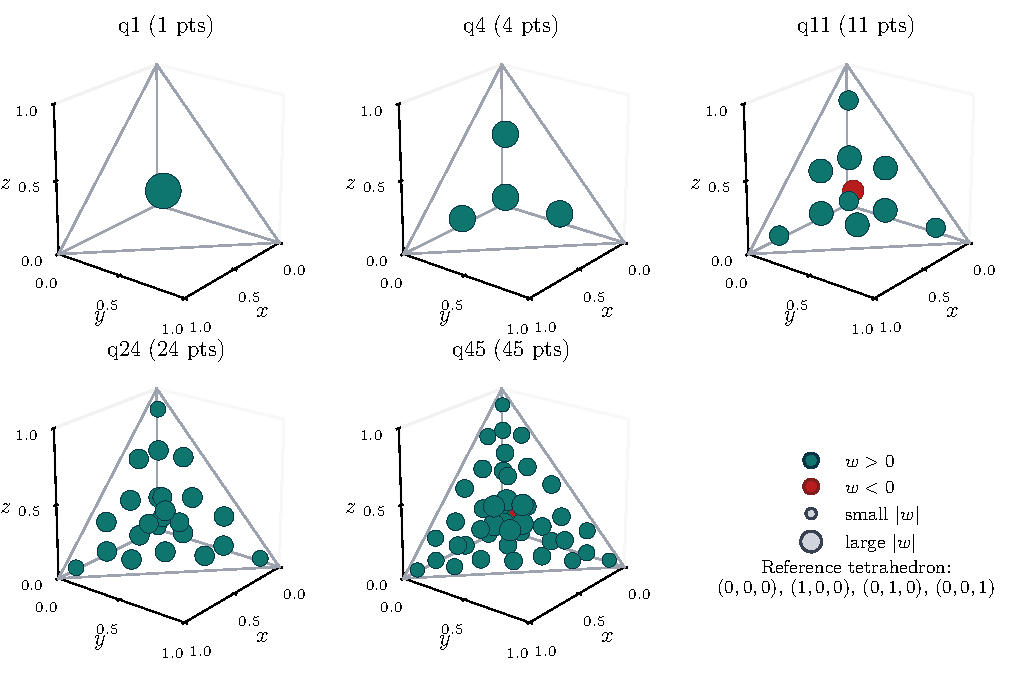
\includegraphics[width=\linewidth,height=0.60\textheight,keepaspectratio]{reference_tetra_quadratures.pdf}
\end{column}
\begin{column}{0.50\textwidth}
\begin{softbox}
\begin{itemize}
  \item The config and element helpers accept \code{P1}, \code{P2}, and \code{P4} on the public interface.
  \item The VTK export path supports \code{VTK\_LAGRANGE\_TETRAHEDRON} for \code{P4}, including correct node ordering.
  \item The postprocess layer adds pointwise deviatoric strain export for 3D \code{P4}, so the higher-order benchmark path can be visualised without dropping back to a low-order fallback.
  \item This matters in practice: higher-order runs, quadrature choice, and the final visual product are now on the public runtime path instead of being one-off utilities.
\end{itemize}
\end{softbox}
\end{column}
\end{columns}
\sourceline{\code{src/slope\_stability/core/elements.py}; \code{src/slope\_stability/postprocess/field\_exports.py}; \code{tests/test\_high\_order\_vtu\_export.py}}
\end{frame}

\SectionDivider{How To Add A New Benchmark}{4}{8}

\begin{frame}{MATLAB Script Versus PETSc Benchmark Folder}
\small
\begin{tabularx}{\textwidth}{p{0.20\textwidth}p{0.31\textwidth}Y}
\toprule
\textbf{Task} & \textbf{MATLAB habit} & \textbf{PETSc rewrite habit} \\
\midrule
Select the runner family & pick a top-level script & copy a benchmark folder and set \code{problem.asset} plus \code{problem.analysis} \\
Select the physics path & change SSR / LL / seepage calls in the script & set \code{problem.analysis}; use \code{continuation.method} only where the runner exposes it \\
Point at the mesh input & edit the loader call inside the script & select \code{problem.mesh\_variant} and optional \code{problem.profile} \\
Define heterogeneity & edit material and conductivity arrays in the script & define materials, mechanics BCs, hydraulics, and seepage BCs in \code{meshes/<asset>/definition.py} \\
Run and inspect outputs & execute the script and keep workspace state alive & run \code{case.toml}, then reuse \code{artifacts/simulation/exports/*} \\
\bottomrule
\end{tabularx}
\end{frame}

\begin{frame}{Benchmark Folder Contract And First Run}
\small
\begin{columns}[T,totalwidth=\textwidth]
\begin{column}{0.47\textwidth}
\miniheading{Bootstrap once}
\begin{pseudobox}
\$ ./bootstrap.sh\\
\$ BOOTSTRAP\_MODE=wheel ./bootstrap.sh
\end{pseudobox}
\miniheading{Folder contract and first run}
\begin{pseudobox}
\code{benchmark\_name/}\\
\code{\ \ case.toml}\\
\code{\ \ run.sh}\\
\code{\ \ README.md}\\
\code{\ \ simulation.ipynb}\\
\code{\ \ visualisation.ipynb}\\[0.10cm]
\$ ./run.sh\\
\$ ./.venv/bin/python -m\\
\ \ slope\_stability.cli.run\_case\_from\_config\\
\ \ benchmarks/<case>/case.toml
\end{pseudobox}
\end{column}
\begin{column}{0.49\textwidth}
\begin{softbox}
\begin{itemize}
  \item \code{case.toml} is the only document the runner consumes directly.
  \item \code{run.sh} is a wrapper around the same config-driven entry point.
  \item \code{README.md} and the notebooks describe or reuse that config; they do not define solver behavior.
  \item Standard outputs land under \code{artifacts/simulation/exports/}; \code{[notebook]} only tunes notebook and display defaults.
\end{itemize}
\end{softbox}
\end{column}
\end{columns}
\end{frame}

\begin{frame}{Choose The Runner Family First}
\small
\begin{tabularx}{\textwidth}{p{0.22\textwidth}p{0.22\textwidth}Y}
\toprule
\textbf{Decision} & \textbf{Typical values} & \textbf{What it actually selects} \\
\midrule
\code{problem.asset} & \code{3d\_hetero\_slope}, \code{3d\_hetero\_seepage} & the registered problem asset and its definition file \\
\code{problem.mesh\_variant} & asset-local \code{.msh} variant & the concrete canonical Gmsh mesh for that asset \\
\code{problem.profile} & \code{fixed\_base}, \code{roller\_base}, or omitted & named mechanics BC overrides from the asset definition \\
\code{problem.analysis} & \code{ssr}, \code{ll}, \code{seepage} & the mechanics, limit-load, or seepage-only route \\
\code{[continuation]}, \code{[newton]}, \code{[linear\_solver]} & numerical controls & solver policy only; not geometry, materials, or hydraulic data \\
\bottomrule
\end{tabularx}
\end{frame}

\begin{frame}{What The Current Public Surface Actually Supports}
\small
\begin{tabularx}{\textwidth}{p{0.24\textwidth}p{0.12\textwidth}p{0.27\textwidth}Y}
\toprule
\textbf{Route style} & \textbf{Analysis} & \textbf{Current continuation surface} & \textbf{Problem input} \\
\midrule
2D mechanics assets & \code{ssr}, \code{ll} & continuation route selected by config & \code{asset}, \code{mesh\_variant}, optional \code{profile} \\
3D mechanics assets & \code{ssr}, \code{ll} & indirect in the current config-driven mainline & \code{asset}, \code{mesh\_variant}, optional \code{profile} \\
Seepage-only assets & \code{seepage} & no continuation branch; seepage and linear-solver blocks drive the solve & seepage spec from \code{definition.py} \\
3D seepage-coupled SSR assets & \code{ssr} & indirect SSR after seepage solve & mechanics and seepage specs from \code{definition.py} \\
\bottomrule
\end{tabularx}
\vspace{0.12cm}
\begin{callout}
\code{case.toml} selects assets and numerical controls. Problem-specific physics belongs in \code{meshes/<asset>/definition.py}.
\end{callout}
\end{frame}

\begin{frame}{Dry Mechanical Example: 3D Heterogeneous SSR}
\small
\begin{columns}[T,totalwidth=\textwidth]
\begin{column}{0.51\textwidth}
\begin{pseudobox}
\code{[problem]}\\
\code{asset = "3d\_hetero\_slope"}\\
\code{mesh\_variant = "adaptive\_family\_a\_l1.msh"}\\
\code{analysis = "ssr"}\\
\code{elem\_type = "P4"}\\[0.10cm]
\code{[execution]}\\
\code{node\_ordering = "block\_metis"}\\[0.10cm]
\code{[continuation]}\\
\code{method = "indirect"}\\
\code{omega\_max = 6.7e6}\\[0.10cm]
\code{[newton]}\\
\code{stopping\_criterion = "absolute\_delta\_lambda"}\\
\code{stopping\_tol = 1e-4}\\[0.10cm]
\code{[linear\_solver]}\\
\code{pc\_backend = "pmg\_shell"}
\end{pseudobox}
\end{column}
\begin{column}{0.45\textwidth}
\begin{softbox}
\begin{itemize}
  \item This selects the 3D dry SSR runner and the current distributed P4/PMG path.
  \item \code{continuation.method = "indirect"} matches the current config-driven 3D mainline.
  \item The mesh variant resolves through \code{meshes/3d\_hetero\_slope/definition.py}; BC labels and materials are asset-owned.
  \item \code{[execution]}, \code{[continuation]}, \code{[newton]}, and \code{[linear\_solver]} own the parallel and solver policy; \code{[notebook]} only affects notebook defaults.
\end{itemize}
\end{softbox}
\end{column}
\end{columns}
\end{frame}

\begin{frame}{Hydro Paths: Seepage Only Versus Seepage-Coupled SSR}
\small
\begin{columns}[T,totalwidth=\textwidth]
\begin{column}{0.48\textwidth}
\miniheading{Seepage-only}
\begin{pseudobox}
\code{[problem]}\\
\code{asset = "3d\_hetero\_seepage"}\\
\code{mesh\_variant = "concave\_family\_b.msh"}\\
\code{analysis = "seepage"}\\
\code{[seepage]}\\
\code{linear\_tolerance = 1e-10}
\end{pseudobox}
\end{column}
\begin{column}{0.48\textwidth}
\miniheading{Seepage-coupled SSR}
\begin{pseudobox}
\code{[problem]}\\
\code{asset = "3d\_hetero\_seepage\_transition"}\\
\code{mesh\_variant = "transition\_default.msh"}\\
\code{profile = "fixed\_base"}\\
\code{analysis = "ssr"}\\
\code{[continuation]}\\
\code{method = "indirect"}
\end{pseudobox}
\end{column}
\end{columns}
\vspace{0.12cm}
\begin{callout}
\code{[seepage]} carries numerical seepage solver tolerances only. Conductivity, water unit weight, and head conditions live in the selected asset definition.
\end{callout}
\end{frame}

\begin{frame}{Boundary Labels, Materials, And 2D Text Meshes}
\small
\begin{columns}[T,totalwidth=\textwidth]
\begin{column}{0.48\textwidth}
\begin{pseudobox}
\code{ASSET = build\_problem\_asset\_3d(}\\
\code{\ \ asset\_id="3d\_hetero\_slope",}\\
\code{\ \ mesh\_variants=\{...\},}\\
\code{\ \ materials=\{...\},}\\
\code{\ \ region\_assignment=\{...\},}\\
\code{\ \ mechanics=\{... profiles ...\},}\\
\code{\ \ seepage=build\_seepage\_spec(...)}\\
\code{)}
\end{pseudobox}
\end{column}
\begin{column}{0.48\textwidth}
\begin{softbox}
\begin{itemize}
  \item Canonical Gmsh physical names use \code{region:*}, \code{boundary:*}, \code{nodeset:*}, and optional \code{boundary\_geom:*}.
  \item The asset API maps regions to material ids and builds mechanics and seepage masks from named targets.
  \item Named profiles replace integer boundary switches such as glued-base or roller-base modes.
  \item \code{case.toml} should not contain raw mesh paths, local material rows, conductivity, water unit weight, or head BCs.
  \item Generic mesh IO reads geometry and labels; problem ownership stays under \code{meshes/<asset>/definition.py}.
\end{itemize}
\end{softbox}
\end{column}
\end{columns}
\end{frame}

\begin{frame}{Benchmark Authoring Checklist}
\small
\begin{enumerate}
  \item Copy the nearest benchmark folder under \code{benchmarks/}, rename it intentionally, and update \code{[benchmark]}.
  \item Set \code{[problem]} first: \code{asset}, \code{mesh\_variant}, optional \code{profile}, \code{analysis}, and \code{elem\_type}.
  \item Put geometry, materials, mechanics BCs, hydraulics, seepage BCs, and profiles in \code{meshes/<asset>/definition.py}.
  \item Fill \code{[execution]}, \code{[continuation]}, \code{[newton]}, and \code{[linear\_solver]}; add \code{[seepage]} only for numerical seepage controls.
  \item Run \code{./run.sh} or \code{run\_case\_from\_config}, then verify \code{artifacts/simulation/exports/*}.
  \item Keep \code{README.md}, \code{simulation.ipynb}, and \code{visualisation.ipynb} aligned with the same \code{case.toml}.
\end{enumerate}
\vspace{0.14cm}
\begin{callout}
A benchmark should remain explainable from \code{case.toml}, \code{meshes/<asset>/definition.py}, and the output folder. If that is no longer true, too much logic has drifted back into hidden runner code.
\end{callout}
\end{frame}

\SectionDivider{Unified Visualisation}{5}{8}

\begin{frame}{Unified Visualisation Pipeline}
\small
\begin{pseudobox}
start\\
$\rightarrow$ solve case\\
$\rightarrow$ write \code{final\_solution.vtu} + debug bundle + history JSON\\
$\rightarrow$ rebuild case mesh from config\\
$\rightarrow$ build standard field exports\\
$\rightarrow$ generated notebooks / PyVista / ParaView consume the same files
\end{pseudobox}
\vspace{0.20cm}
\begin{columns}[T,totalwidth=\textwidth]
\begin{column}{0.49\textwidth}
\begin{softbox}
\miniheading{Key rewrite helpers}
\begin{itemize}
  \item \code{postprocess/case\_mesh.py}
  \item \code{postprocess/field\_exports.py}
  \item \code{benchmarks/notebook\_support.py}
\end{itemize}
\end{softbox}
\end{column}
\begin{column}{0.49\textwidth}
\begin{softbox}
\miniheading{Result}
\begin{itemize}
  \item one mesh reconstruction surface
  \item one field naming surface
  \item one notebook generation surface
  \item one export surface for external viewers
\end{itemize}
\end{softbox}
\end{column}
\end{columns}
\sourceline{\code{src/slope\_stability/postprocess/case\_mesh.py}; \code{src/slope\_stability/postprocess/field\_exports.py}; \code{benchmarks/notebook\_support.py}}
\end{frame}

\begin{frame}{PETSc 3D Views: Geometry And Warped Displacement}
\small
\begin{columns}[T,totalwidth=\textwidth]
\begin{column}{0.49\textwidth}
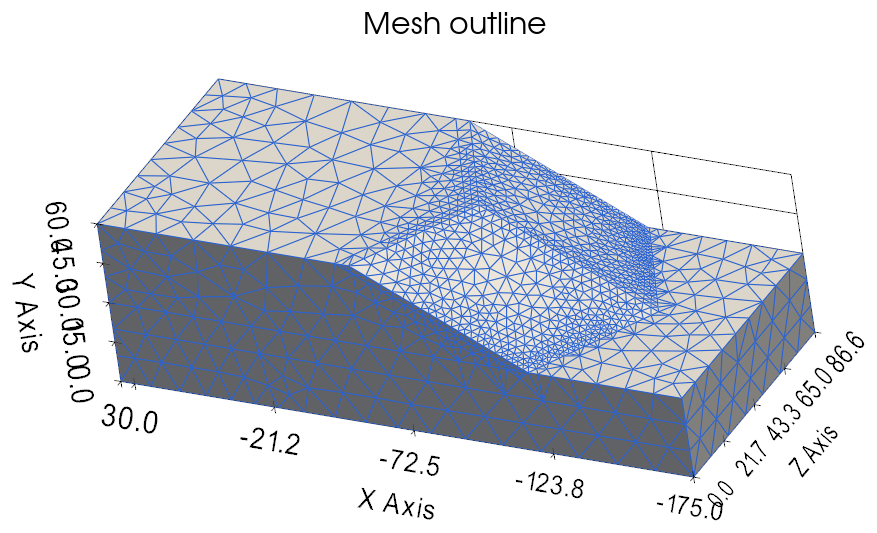
\includegraphics[width=\linewidth,height=0.48\textheight,keepaspectratio]{petsc_geometry_current.png}
\end{column}
\begin{column}{0.49\textwidth}
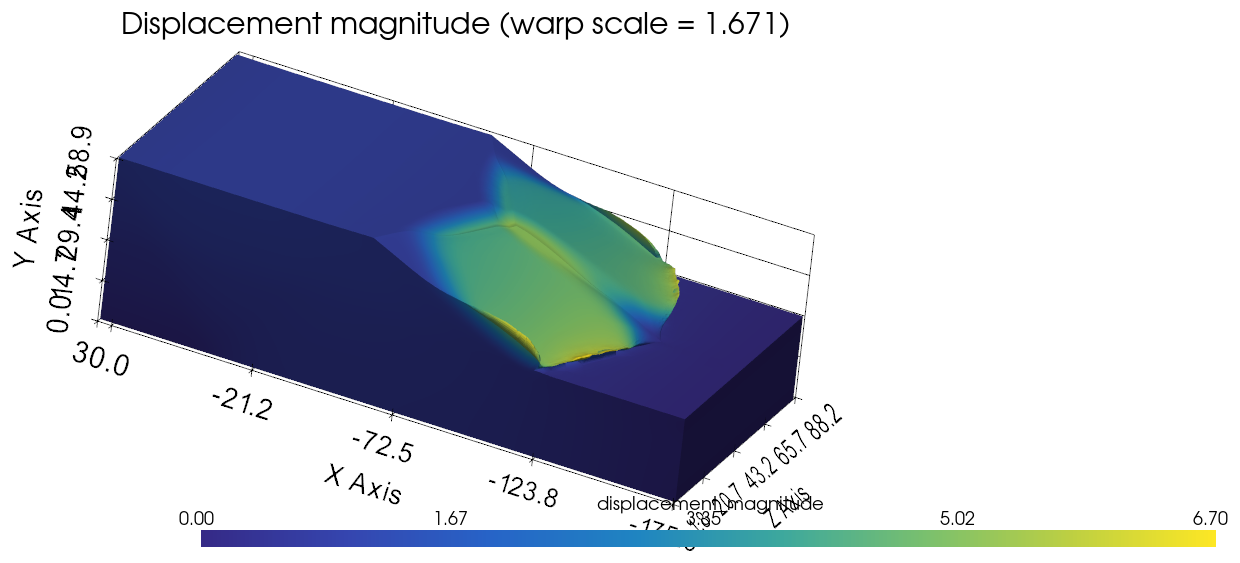
\includegraphics[width=\linewidth,height=0.48\textheight,keepaspectratio]{petsc_displacement_current.png}
\end{column}
\end{columns}
\vspace{0.12cm}
\begin{softbox}
\begin{itemize}
  \item Both panels are taken from the default indirect 3D SSR visualisation notebook path.
  \item Left: mesh-outline view showing the local refinement pattern.
  \item Right: warped displacement view from the same benchmark and the same exported solution bundle.
\end{itemize}
\end{softbox}
\end{frame}

\begin{frame}{PETSc Localisation Surface And Top-View Slices}
\small
\begin{columns}[T,totalwidth=\textwidth]
\begin{column}{0.42\textwidth}
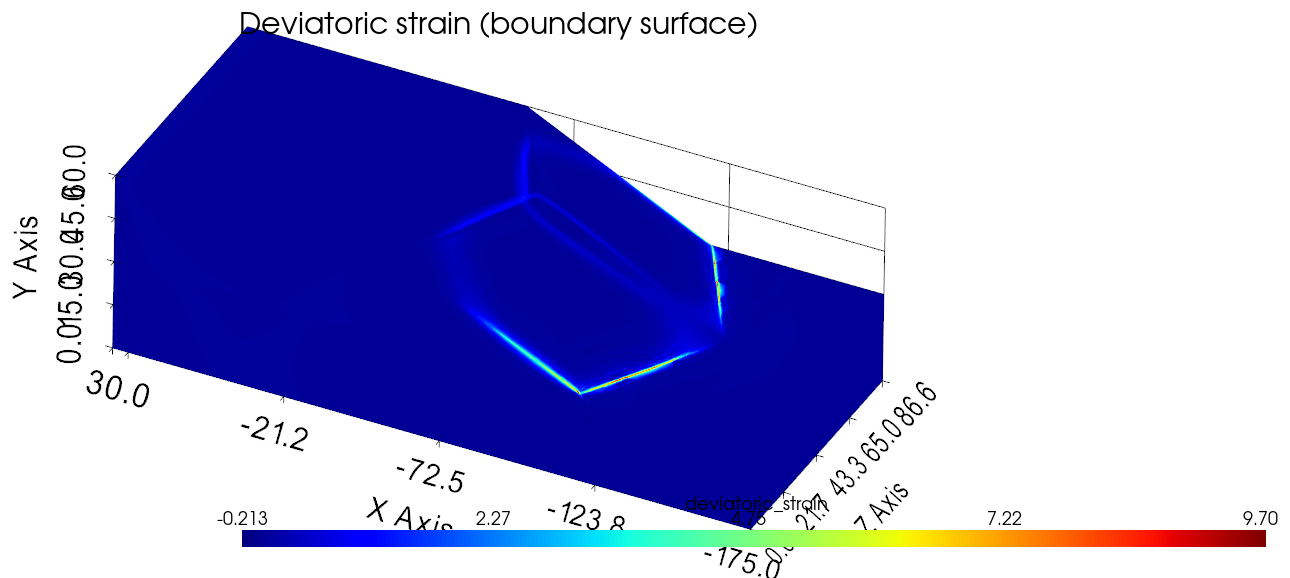
\includegraphics[width=\linewidth,height=0.46\textheight,keepaspectratio]{petsc_deviatoric_surface_current.png}
\end{column}
\begin{column}{0.55\textwidth}
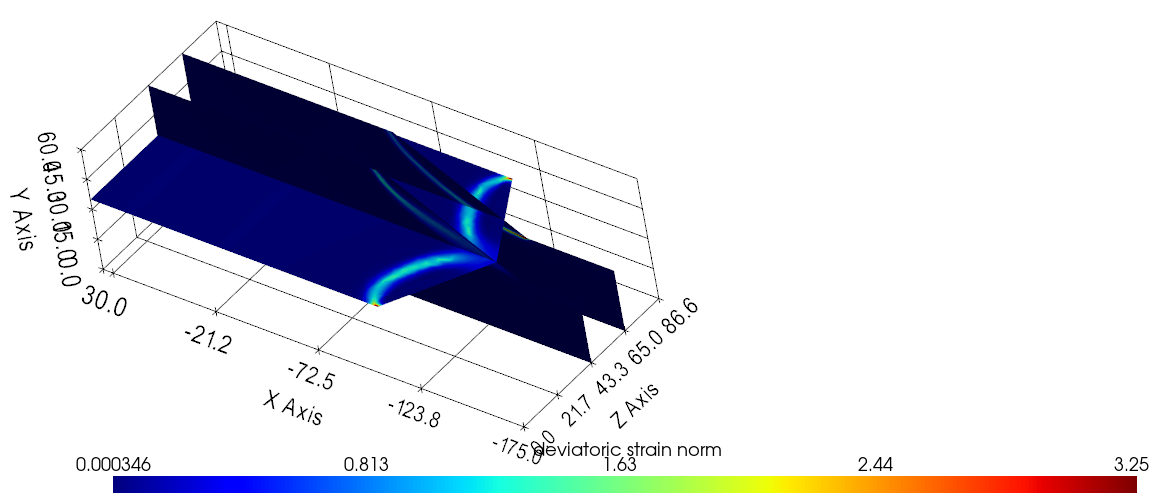
\includegraphics[width=\linewidth,height=0.46\textheight,keepaspectratio]{petsc_slices_current.png}
\end{column}
\end{columns}
\vspace{0.16cm}
\begin{softbox}
\begin{itemize}
  \item Both panels come from the same default indirect visualisation path and the same exported \code{deviatoric\_strain} field.
  \item The 3D panel keeps the notebook-style full boundary-surface view that the authors are already used to reading.
  \item The slice panel stays a real top-view cut product at the benchmark-configured planes, with the same capped warm-to-cool scale used in the 3D deviatoric view shown on the left.
\end{itemize}
\end{softbox}
\end{frame}

\begin{frame}{MATLAB And PETSc Reach Similar Slice Products Through Different Workflows}
\small
\begin{columns}[T,totalwidth=\textwidth]
\begin{column}{0.49\textwidth}
\miniheading{MATLAB}
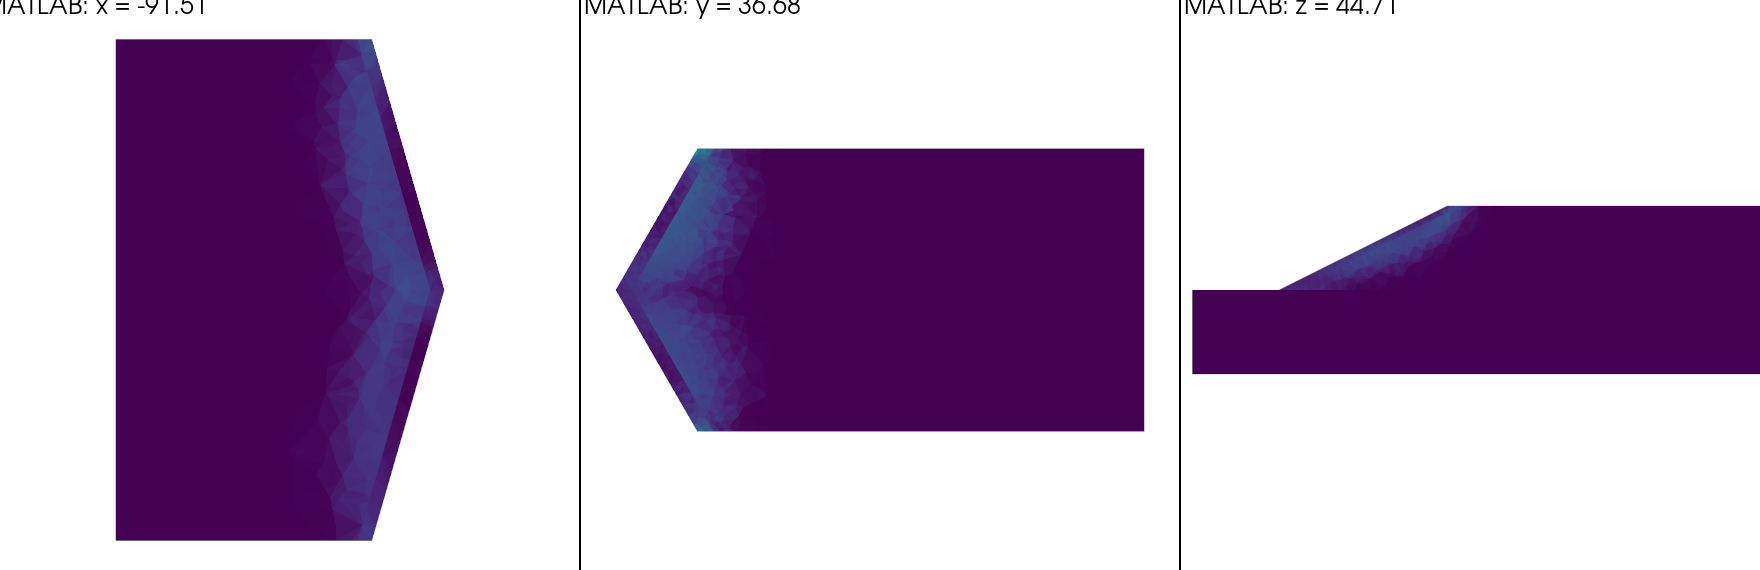
\includegraphics[width=\linewidth,height=0.40\textheight,keepaspectratio]{matlab_slices_present.png}
\end{column}
\begin{column}{0.49\textwidth}
\miniheading{PETSc rewrite}
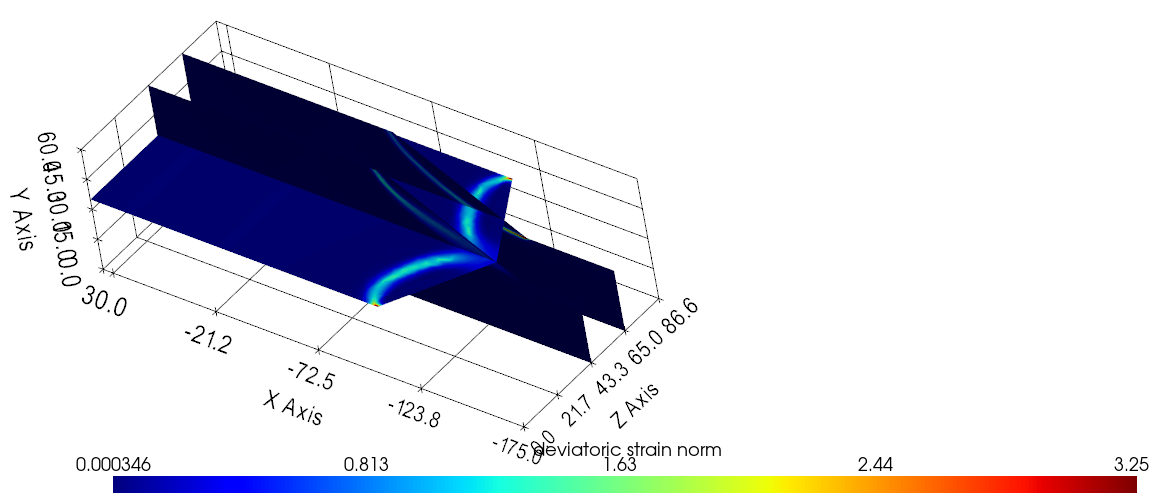
\includegraphics[width=\linewidth,height=0.40\textheight,keepaspectratio]{petsc_slices_current.png}
\end{column}
\end{columns}
\vspace{0.14cm}
\begin{callout}
The visual end product stays familiar. The production path changes: MATLAB builds the slice product in the case script, while the rewrite rebuilds it from shared exports and shared notebook support.
\end{callout}
\end{frame}

\SectionDivider{Unified Meshes}{6}{8}

\begin{frame}{MATLAB Mesh Handling And Element Degree Are Entangled}
\small
\begin{tabularx}{\textwidth}{p{0.28\textwidth}p{0.27\textwidth}Y}
\toprule
\textbf{Question} & \textbf{MATLAB answer} & \textbf{Consequence} \\
\midrule
Mesh storage choice & Usually a degree-specific loader & Mesh storage and FE order drift together \\
Higher-order support path & Build new midpoint utilities and matching assumptions & Higher order grows sideways by utility proliferation \\
Material and BC interpretation & Inside the case loader path & Harder to reuse across benchmark families \\
Free-mask source & Loader-specific face conventions & Less separation between geometry and solve policy \\
\bottomrule
\end{tabularx}
\sourceline{\code{slope\_stability\_matlab/+MESH/load\_mesh\_P2.m}; \code{slope\_stability\_matlab/+MESH/midpoints\_P4.m}}
\end{frame}

\begin{frame}{PETSc Mesh Families Carry Their Own Metadata}
\small
\begin{columns}[T,totalwidth=\textwidth]
\begin{column}{0.52\textwidth}
\begin{pseudobox}
\code{ASSET = build\_problem\_asset\_3d(}\\
\code{  asset\_id="3d\_hetero\_slope",}\\
\code{  default\_variant="adaptive\_family\_a\_l1.msh",}\\
\code{  mesh\_variants=\{...\},}\\
\code{  mechanics=\{profiles, materials, BCs\}}\\
\code{)}
\code{\}}
\end{pseudobox}
\end{column}
\begin{column}{0.44\textwidth}
\begin{softbox}
\begin{itemize}
  \item Each asset declares mesh variants, profiles, boundary labels, materials, and hydraulics.
  \item The case config selects the asset, mesh variant, optional profile, analysis, and solver settings.
  \item The runtime receives reusable asset data, not problem-specific source modules.
\end{itemize}
\end{softbox}
\end{column}
\end{columns}
\sourceline{\code{meshes/3d\_hetero\_slope/definition.py}; \code{src/slope\_stability/assets/}}
\end{frame}

\begin{frame}{Mesh Family And \code{elem\_type} Are Now Separate Concepts}
\small
\begin{tabularx}{\textwidth}{p{0.30\textwidth}p{0.25\textwidth}Y}
\toprule
\textbf{Concept} & \textbf{Where it lives} & \textbf{Meaning} \\
\midrule
Mesh family & \code{meshes/*/definition.py} + canonical \code{.msh} files & Geometry, physical tags, default material metadata \\
\code{problem.mesh\_path} & \code{case.toml} & Which family member or external mesh file to load \\
\code{problem.elem\_type} & \code{case.toml} & Which FE degree the runtime should use on that mesh \\
Loader/elevation path & \code{io.py} + \code{mesh/loader.py} & How the runtime lifts canonical tet4 storage to \code{P1}, \code{P2}, or \code{P4} \\
\bottomrule
\end{tabularx}
\vspace{0.18cm}
\begin{callout}
This is the core 3D mesh design change: \term{geometry/material family selection} and \term{finite-element degree selection} are no longer the same decision.
\end{callout}
\sourceline{\code{src/slope\_stability/core/elements.py}; \code{src/slope\_stability/problem\_assets.py}; \code{docs/config\_case\_matrix.md}}
\end{frame}

\begin{frame}{Boundary Tags, Material Tags, And Reordering Stay Explicit}
\small
\begin{columns}[T,totalwidth=\textwidth]
\begin{column}{0.32\textwidth}
\MetricTile{Boundary labels}{
Mesh-family metadata declares which physical labels correspond to constrained \(x\), \(y\), and \(z\) directions.
}
\end{column}
\begin{column}{0.32\textwidth}
\MetricTile{Material identifiers}{
Element-wise material ids stay attached to the mesh and can be expanded into integration-point rows later.
}
\end{column}
\begin{column}{0.32\textwidth}
\MetricTile{Node reorder}{
The same mesh can then be reordered for ownership without losing its physical meaning.
}
\end{column}
\end{columns}
\vspace{0.20cm}
\begin{softbox}
The rewrite does not hide physics labels behind generic partitioning. It keeps labels explicit, then reorders the discrete system around them.
\end{softbox}
\sourceline{\code{meshes/3d\_hetero\_ssr/definition.py}; \code{src/slope\_stability/mesh/reorder.py}; \code{docs/petsc\_matlab\_map/chapters/mainline/02\_mesh\_materials\_load.tex}}
\end{frame}

\SectionDivider{Speed Comparison}{7}{8}

\begin{frame}{Locked Runtime Study Protocol}
\small
\begin{softbox}
\begin{itemize}
  \item The committed PETSc-vs-MATLAB performance report uses indirect SSR only and \code{P2} elements only.
  \item PETSc runs use \code{mpirun -n 8} with \code{OMP\_NUM\_THREADS = 1}.
  \item MATLAB runs use \code{OMP\_NUM\_THREADS = 8} with the BoomerAMG MATLAB path on 8 threads.
  \item The three primary cases are homogeneous 3D SSR, heterogeneous 3D SSR, and heterogeneous 3D seepage SSR.
  \item The study is sequential and normalised into CSV before figures and tables are built.
\end{itemize}
\end{softbox}
\vspace{0.18cm}
\begin{callout}
The study answers ``how does the committed P2 PETSc implementation compare under this controlled protocol?'' It does \textbf{not} directly answer ``how fast is the current default P4 architecture path?''.
\end{callout}
\datasourceline{\code{docs/petsc\_matlab\_performance\_comparison}: README and main LaTeX report}
\end{frame}

\begin{frame}{Locked P2 Study: Headline View Across The Three Cases}
\small
\begin{tabularx}{\textwidth}{p{0.27\textwidth}p{0.16\textwidth}p{0.15\textwidth}Y}
\toprule
\textbf{Case} & \textbf{Levels} & \textbf{M/P gap} & \textbf{Headline} \\
\midrule
Homogeneous 3D SSR & L1 to L4 & \(1.24\times\) to \(3.47\times\) & PETSc pulls further ahead as the dry mesh ladder grows. \\
Heterogeneous 3D SSR & L1 to L4 & \(1.35\times\) to \(3.08\times\) & Same trend on the dry case closest to the architecture anchor. \\
Heterogeneous 3D seepage SSR & \code{concave\_L2} only & \(2.02\times\) & Positive completed level, but the next level remains part of the reported limitation. \\
\bottomrule
\end{tabularx}
\datasourceline{committed \code{P2} study generated tables in \code{docs/petsc\_matlab\_performance\_comparison/generated}}
\end{frame}

\begin{frame}{Homogeneous 3D SSR: PETSc Pulls Ahead As The Mesh Grows}
\small
\begin{columns}[T,totalwidth=\textwidth]
\begin{column}{0.49\textwidth}
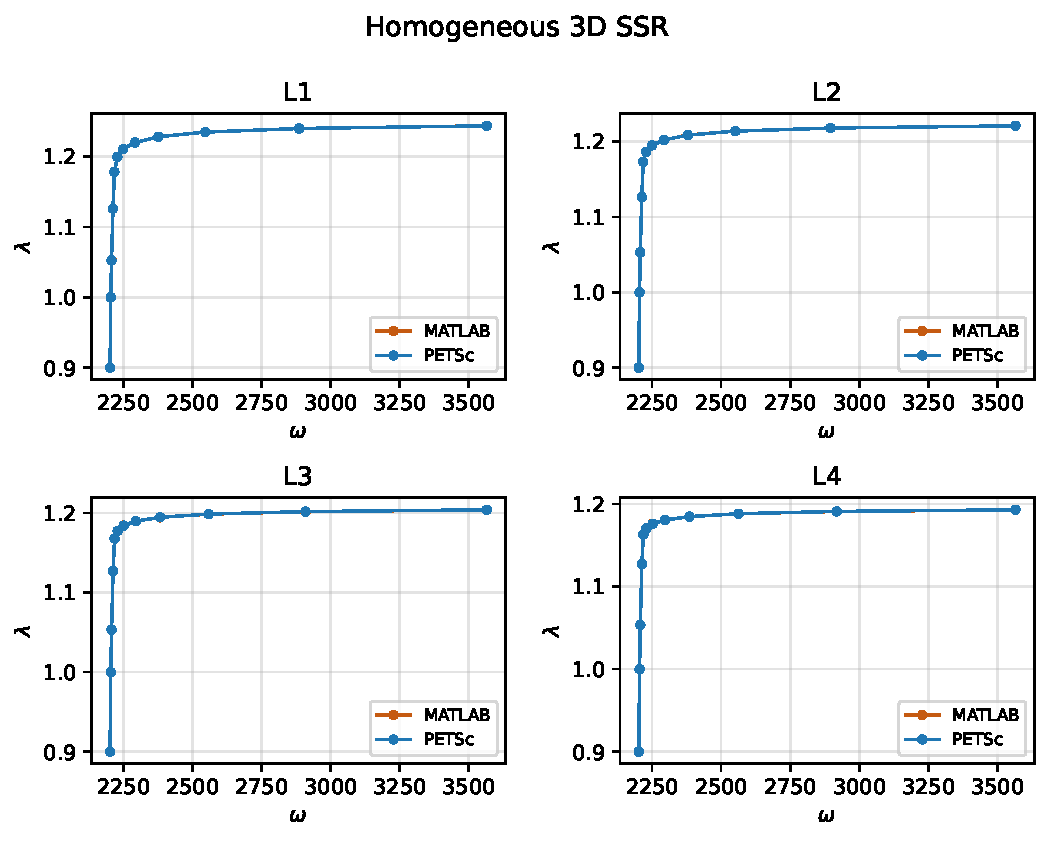
\includegraphics[width=\linewidth,height=0.50\textheight,keepaspectratio]{homo_3d_continuation.pdf}
\end{column}
\begin{column}{0.49\textwidth}
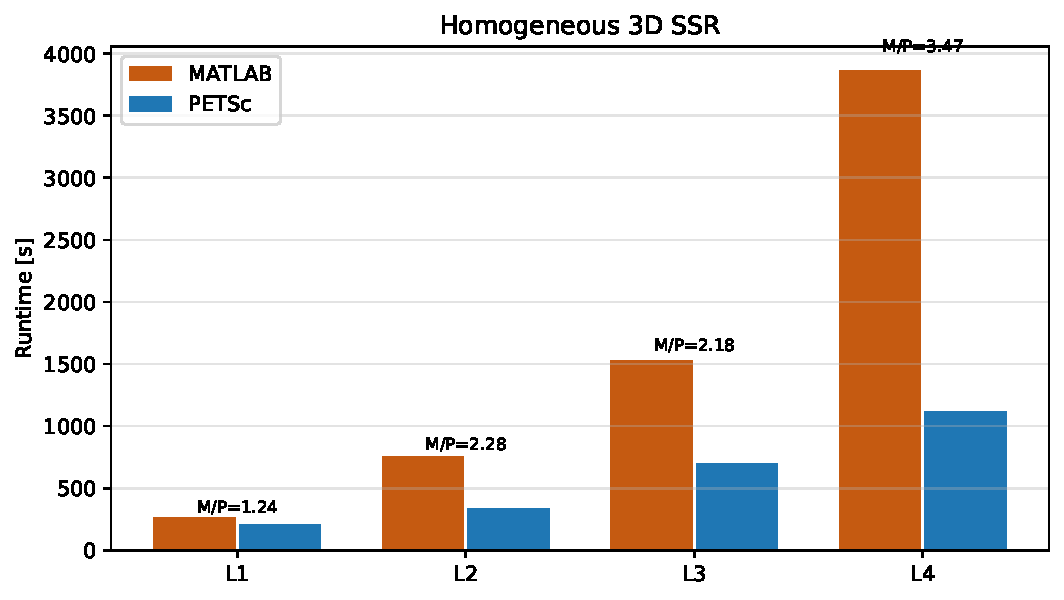
\includegraphics[width=\linewidth,height=0.50\textheight,keepaspectratio]{homo_3d_timings.pdf}
\end{column}
\end{columns}
\vspace{0.14cm}
\begin{softbox}
\begin{itemize}
  \item PETSc runtime goes from \(210.5\) s at L1 to \(1115.2\) s at L4.
  \item MATLAB runtime goes from \(261.8\) s at L1 to \(3865.1\) s at L4.
  \item The MATLAB-over-PETSc ratio grows from \(1.24\times\) to \(3.47\times\).
\end{itemize}
\end{softbox}
\datasourceline{\code{presentation\_petsc\_rewrite/assets}: homogeneous 3D continuation and timings from the committed study}
\end{frame}

\begin{frame}{Homogeneous 3D SSR: Committed P2 Ladder Versus The New P4(L1) Curve}
\small
\centering
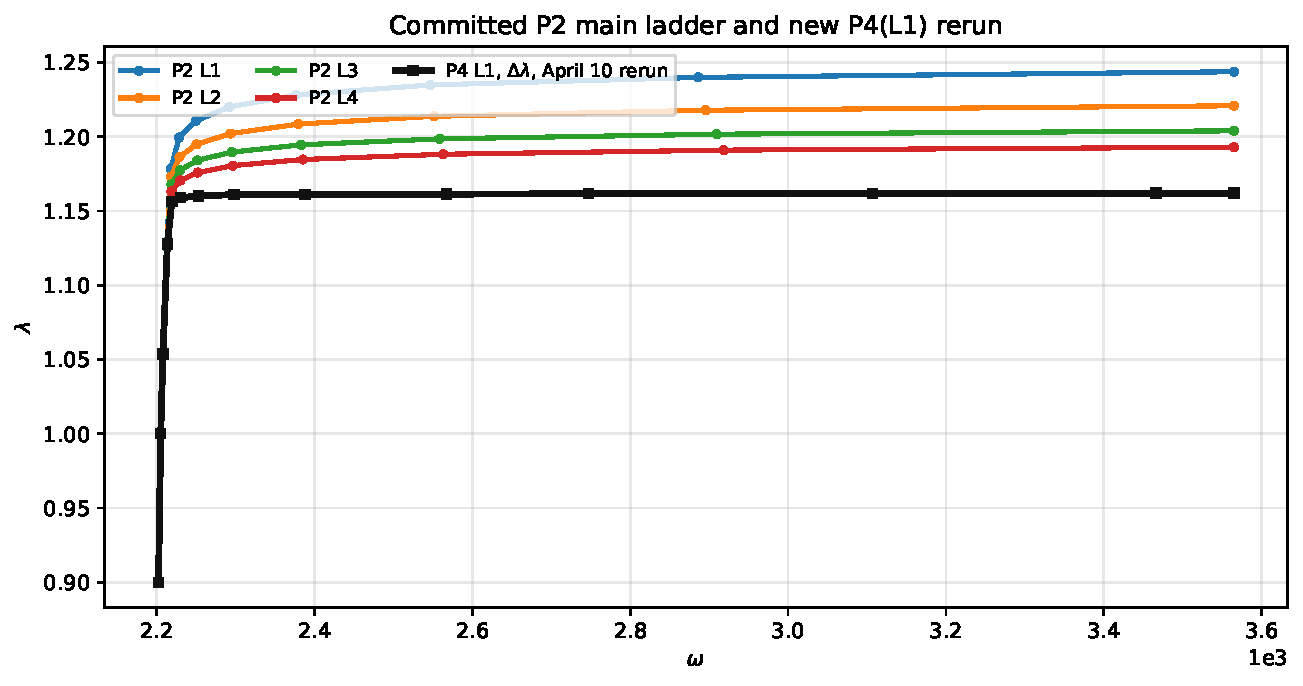
\includegraphics[width=\linewidth,height=0.46\textheight,keepaspectratio]{homo_3d_p2_vs_p4_curves.pdf}
\vspace{0.12cm}
\begin{softbox}
\begin{itemize}
  \item Every colored line is an available committed PETSc \code{P2} study run for this case.
  \item The black line is the April 10 rerun on \code{P4(L1)} with the fixed PMG shell, \(\Delta\lambda\) stop, and the same \(\omega_{\max}\) as the committed study.
  \item This slide compares continuation shape under a higher-order discretisation, not runtime parity with the committed \code{P2} protocol.
\end{itemize}
\end{softbox}
\datasourceline{committed \code{docs/petsc\_matlab\_performance\_comparison/data/continuation\_curves.csv} plus April 10, 2026 rerun artifacts in \code{artifacts/comparisons/p4\_l1\_vs\_p2\_presentation\_20260410}}
\end{frame}

\begin{frame}{Heterogeneous 3D SSR: Same Trend, Stronger Advantage On Larger Levels}
\small
\begin{columns}[T,totalwidth=\textwidth]
\begin{column}{0.49\textwidth}
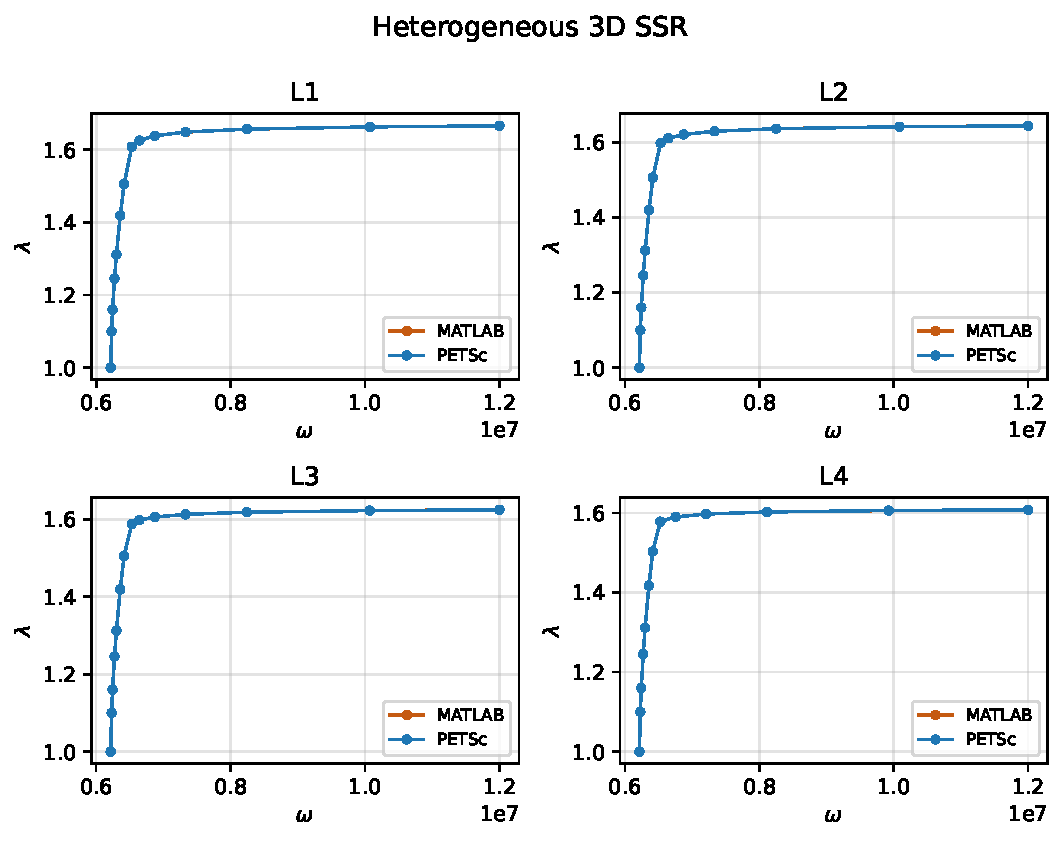
\includegraphics[width=\linewidth,height=0.50\textheight,keepaspectratio]{hetero_3d_continuation.pdf}
\end{column}
\begin{column}{0.49\textwidth}
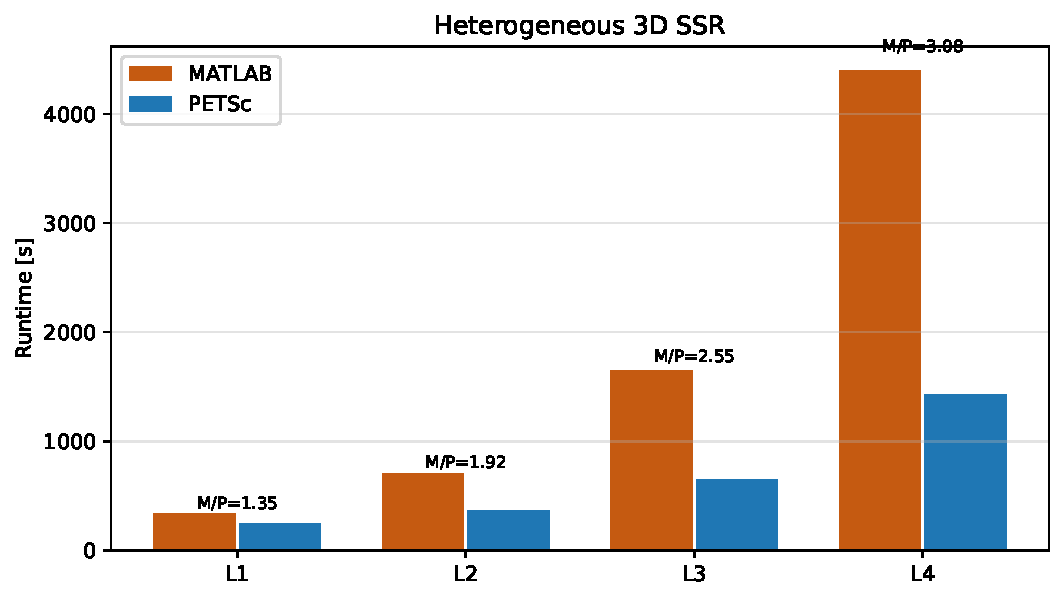
\includegraphics[width=\linewidth,height=0.50\textheight,keepaspectratio]{hetero_3d_timings.pdf}
\end{column}
\end{columns}
\vspace{0.14cm}
\begin{softbox}
\begin{itemize}
  \item PETSc runtime grows from \(247.3\) s at L1 to \(1430.2\) s at L4.
  \item MATLAB runtime grows from \(334.2\) s at L1 to \(4399.1\) s at L4.
  \item The MATLAB-over-PETSc ratio grows from \(1.35\times\) to \(3.08\times\).
\end{itemize}
\end{softbox}
\datasourceline{\code{presentation\_petsc\_rewrite/assets}: heterogeneous 3D continuation and timings from the committed study}
\end{frame}

\begin{frame}{Heterogeneous 3D SSR: Where The New P4(L1) Curve Sits Relative To P2}
\small
\centering
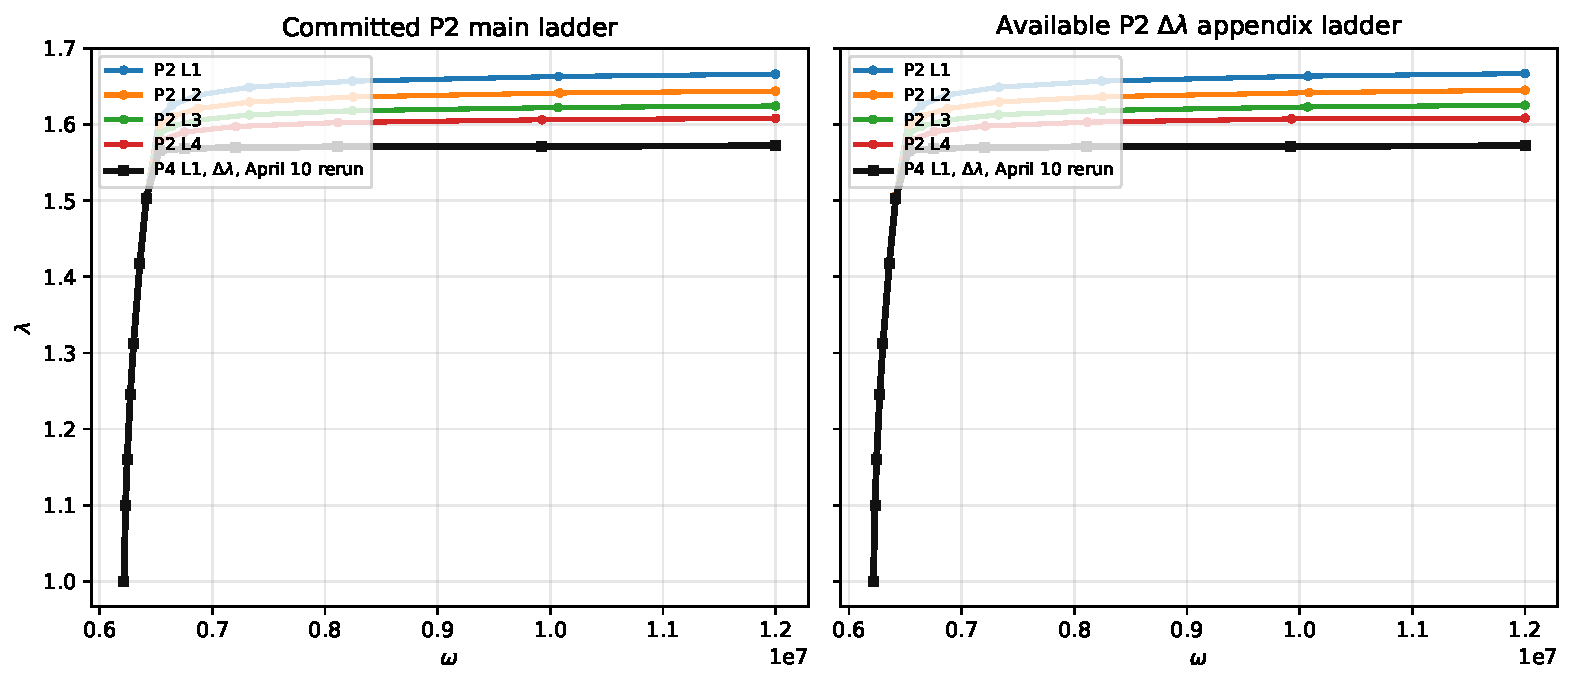
\includegraphics[width=\linewidth,height=0.46\textheight,keepaspectratio]{hetero_3d_p2_vs_p4_curves.pdf}
\vspace{0.12cm}
\begin{softbox}
\begin{itemize}
  \item Left: committed \code{P2} main ladder. Right: available \(\Delta\lambda\) appendix ladder for the same dry heterogeneous case.
  \item The black line is the new \code{P4(L1)} rerun with the fixed PMG shell, \(\Delta\lambda = 10^{-4}\), and the same \(\omega_{\max} = 1.2\times 10^{7}\).
\end{itemize}
\end{softbox}
\datasourceline{committed \code{docs/petsc\_matlab\_performance\_comparison/data/continuation\_curves.csv} plus April 10, 2026 rerun artifacts in \code{artifacts/comparisons/p4\_l1\_vs\_p2\_presentation\_20260410}}
\end{frame}

\begin{frame}{Seepage 3D SSR: Only One Level Completed Under The Locked Protocol}
\small
\begin{columns}[T,totalwidth=\textwidth]
\begin{column}{0.49\textwidth}
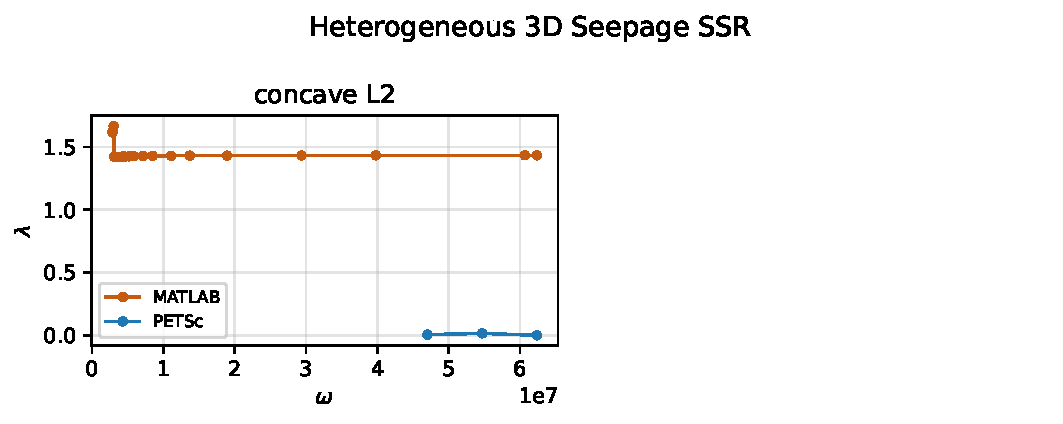
\includegraphics[width=\linewidth,height=0.50\textheight,keepaspectratio]{seepage_3d_continuation.pdf}
\end{column}
\begin{column}{0.49\textwidth}
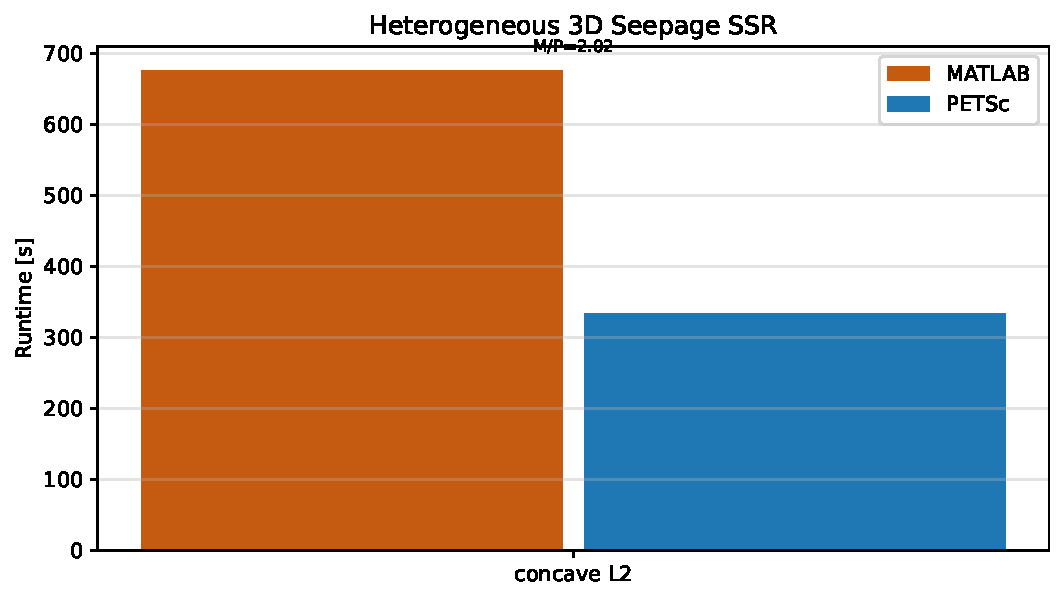
\includegraphics[width=\linewidth,height=0.50\textheight,keepaspectratio]{seepage_3d_timings.pdf}
\end{column}
\end{columns}
\vspace{0.14cm}
\begin{softbox}
\begin{itemize}
  \item On \code{concave\_L2}, PETSc finished in \(334.1\) s and MATLAB in \(676.3\) s, a \(2.02\times\) advantage.
  \item Only this level completed under the committed mixed PMG-shell seepage study protocol.
  \item On this host, the local P4 rerun exceeded available memory during the SSR phase; the slide therefore keeps the committed P2 seepage evidence and marks P4 as skipped locally.
\end{itemize}
\end{softbox}
\datasourceline{\code{presentation\_petsc\_rewrite/assets}: seepage 3D continuation and timings from the committed study}
\end{frame}

\begin{frame}{Additional Speedup Gain: The Delta-Lambda Stop Rule}
\small
\begin{columns}[T,totalwidth=\textwidth]
\begin{column}{0.49\textwidth}
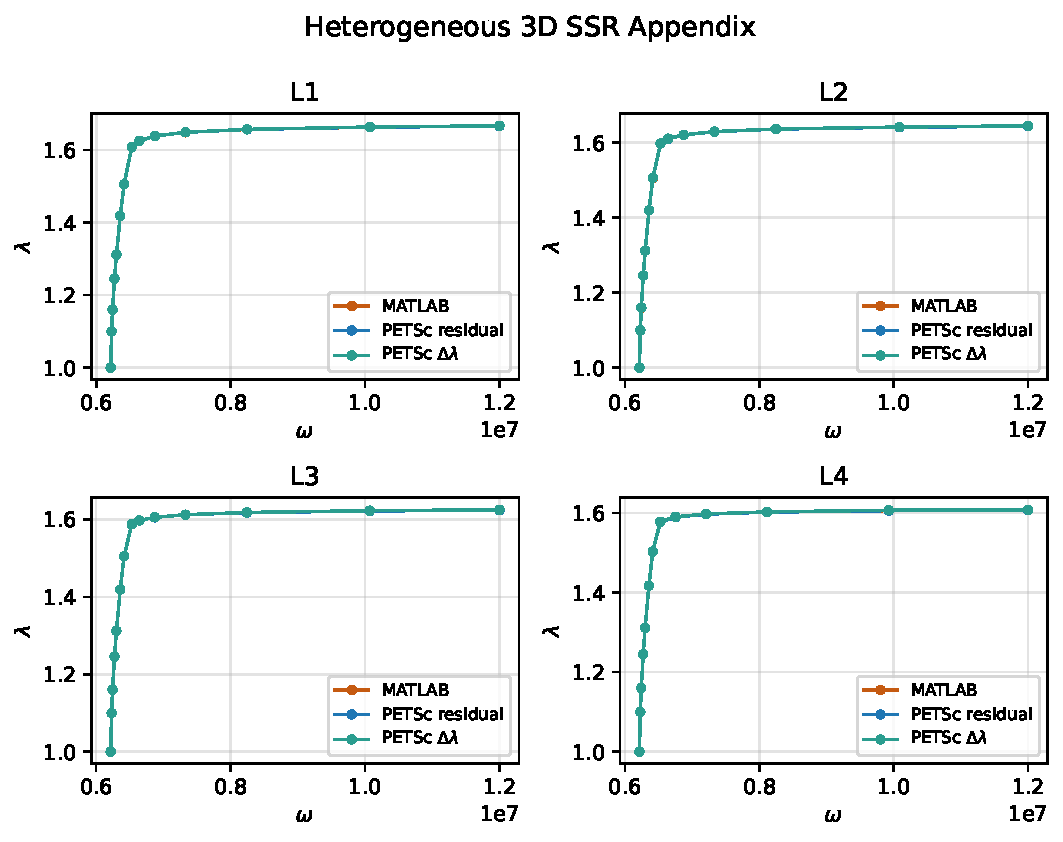
\includegraphics[width=\linewidth,height=0.40\textheight,keepaspectratio]{hetero_3d_delta_lambda_continuation.pdf}
\end{column}
\begin{column}{0.49\textwidth}
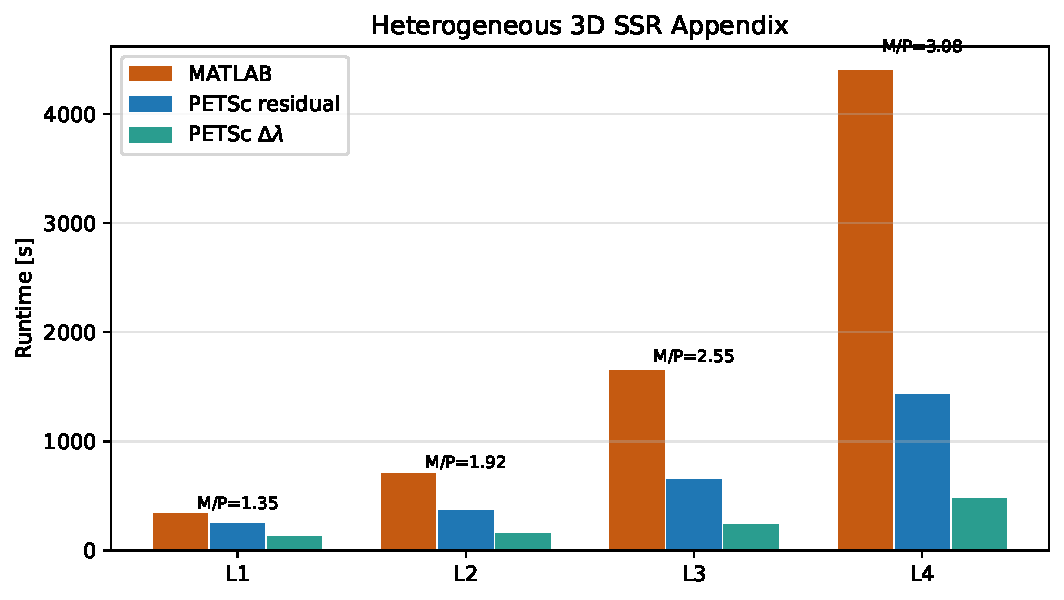
\includegraphics[width=\linewidth,height=0.40\textheight,keepaspectratio]{hetero_3d_delta_lambda_timings.pdf}
\end{column}
\end{columns}
\vspace{0.10cm}
\begin{columns}[T,totalwidth=\textwidth]
\begin{column}{0.52\textwidth}
\begin{softbox}
\begin{itemize}
  \item On the same heterogeneous dry study, the \(\Delta\lambda\) stop rule is \(2.0\times\) faster than the residual baseline at L1 and \(3.0\times\) faster at L4.
  \item Against MATLAB, that pushes the gap from \(2.7\times\) at L1 to \(9.3\times\) at L4.
\end{itemize}
\end{softbox}
\end{column}
\begin{column}{0.44\textwidth}
\begin{callout}
This is a controlled ``other speedup gain'' slide. The study branch stays the same; only the stop policy changes.
\end{callout}
\end{column}
\end{columns}
\datasourceline{\code{docs/petsc\_matlab\_performance\_comparison}: delta-lambda figures and generated table}
\end{frame}

\SectionDivider{Where To Edit The Code And Close}{8}{8}

\begin{frame}{Code Entry Points For Common Changes}
\small
\begin{tabularx}{\textwidth}{p{0.34\textwidth}Y}
\toprule
\textbf{Question} & \textbf{Primary entry point} \\
\midrule
Create or edit a benchmark & \code{benchmarks/*/case.toml}, then \code{src/slope\_stability/core/run\_config.py}, then \code{src/slope\_stability/cli/run\_case\_from\_config.py} \\
Where do mesh, BC labels, and default materials live? & \code{meshes/*/definition.py} plus \code{src/slope\_stability/problem\_assets.py} \\
Change constitutive behavior & \code{src/slope\_stability/constitutive/problem.py} and \code{src/slope\_stability/constitutive/reduction.py} \\
Change Newton or line search & \code{src/slope\_stability/nonlinear/newton.py} and \code{src/slope\_stability/nonlinear/damping.py} \\
Change continuation logic & \code{src/slope\_stability/continuation/indirect.py}, \code{direct.py}, \code{limit\_load.py} \\
Change exports or notebooks & \code{src/slope\_stability/postprocess/*} and \code{benchmarks/notebook\_support.py} \\
\bottomrule
\end{tabularx}
\end{frame}

\begin{frame}{Algorithm Changes Live In A Few Concentrated Files}
\small
\begin{tabularx}{\textwidth}{p{0.30\textwidth}Y}
\toprule
\textbf{Area} & \textbf{Main edit surface} \\
\midrule
Constitutive law & \code{constitutive/problem.py} for stress/tangent logic and \code{constitutive/reduction.py} for Davis reduction \\
Newton solve & \code{nonlinear/newton.py} for SSR and LL Newton kernels; \code{nonlinear/damping.py} for damping and Armijo logic \\
Continuation policy & \code{continuation/indirect.py}, \code{continuation/direct.py}, and \code{continuation/limit\_load.py} \\
Linear solver / PMG & \code{linear/solver.py} and \code{linear/pmg.py} \\
Runner-side assembly and problem wiring & \code{execution/asset\_case/runner.py} dispatching to generic mechanics or seepage runners \\
Postprocess / visualisation & \code{postprocess/case\_mesh.py}, \code{postprocess/field\_exports.py}, and \code{benchmarks/notebook\_support.py} \\
\bottomrule
\end{tabularx}
\end{frame}

\begin{frame}{Final Summary}
\small
\begin{columns}[T,totalwidth=\textwidth]
\begin{column}{0.32\textwidth}
\MetricTile{What stayed familiar}{
SSR, Newton, constitutive reduction, and the benchmark families remain structurally familiar.
}
\end{column}
\begin{column}{0.32\textwidth}
\MetricTile{What changed in the runtime}{
Configuration, ownership-aware assembly, solver separation, standard exports, and shared notebooks are now first-class interfaces.
}
\end{column}
\begin{column}{0.32\textwidth}
\MetricTile{Shortest path to extension}{
Extension now starts from the benchmark folder, mesh-family metadata, concentrated algorithm files, and standard outputs instead of one large script.
}
\end{column}
\end{columns}
\end{frame}

\appendix
\AppendixDivider{Optional Paths, Caveats, And Additional Reading}

\begin{frame}{Architecture Mainline Versus Performance Study Protocol}
\small
\begin{tabularx}{\textwidth}{p{0.28\textwidth}p{0.26\textwidth}Y}
\toprule
\textbf{Question} & \textbf{Architecture mainline} & \textbf{Committed performance study} \\
\midrule
Purpose & Explain the current rewrite structure & Compare PETSc and MATLAB under one locked protocol \\
Case anchor & \code{default P4 benchmark} & \code{committed P2 report} \\
Element degree & \code{P4} default path & \code{P2} only \\
Solver backend focus & \code{pmg\_shell}, owned-row path & PETSc MPI-8 versus MATLAB OMP-8 \\
What it proves & How the rewrite is structured today & How one committed PETSc branch compares numerically and in runtime \\
\bottomrule
\end{tabularx}
\end{frame}

\begin{frame}{Optional And Inactive Paths Present In The Repository}
\small
\begin{softbox}
\begin{itemize}
  \item Direct SSR and LL continuation remain present and runnable for selected cases.
  \item BDDC, Hypre, GAMG, and multiple PMG variants all exist as selectable branches.
  \item Different constitutive ownership modes remain available beyond the overlap mainline.
  \item The map document keeps these paths in its annex so they do not distort the default-reading story.
\end{itemize}
\end{softbox}
\sourceline{\code{docs/petsc\_matlab\_map/chapters/annex/*}; \code{src/slope\_stability/continuation/*}; \code{src/slope\_stability/linear/*}}
\end{frame}

\begin{frame}{Global Assembly And The Legacy Tangent Kernel}
\small
\begin{tabularx}{\textwidth}{p{0.26\textwidth}p{0.26\textwidth}Y}
\toprule
\textbf{Path} & \textbf{Still present?} & \textbf{Why it is not the default story} \\
\midrule
Global \code{B' D B} rebuild & yes & It matches the old MATLAB intuition better, but it is not the normal owned-row PMG route \\
Legacy tangent kernel & yes & Kept for comparison and fallback, but the \code{rows} kernel is the production default for the mainline path \\
Legacy scatter-style assembly & yes & Appendix material now that overlap-owned assembly is the default architectural choice \\
\bottomrule
\end{tabularx}
\sourceline{\code{docs/petsc\_matlab\_map/chapters/annex/05\_tangent\_assembly.tex}; \code{src/slope\_stability/fem/distributed\_tangent.py}}
\end{frame}

\begin{frame}{Alternative Linear-Solver Branches}
\small
\begin{tabularx}{\textwidth}{p{0.22\textwidth}p{0.20\textwidth}Y}
\toprule
\textbf{Branch} & \textbf{Repository status} & \textbf{Typical reason to look at it} \\
\midrule
\code{hypre} backend & active & Classical AMG comparison against PMG-shell \\
\code{gamg} backend & active & PETSc-native algebraic multigrid studies \\
\code{bddc} backend & active & Domain decomposition experiments and MATIS-style subdomain work \\
\code{DIRECT} & active but non-mainline & Small-case validation, not distributed production solves \\
\bottomrule
\end{tabularx}
\sourceline{\code{src/slope\_stability/linear/solver.py}; \code{tests/test\_solver\_preconditioner\_policies.py}}
\end{frame}

\begin{frame}{Seepage Caveat In The Committed Performance Report}
\small
\begin{softbox}
\begin{itemize}
  \item The seepage section reports only \code{concave\_L2}.
  \item The next seepage level reproduced a PETSc-side crash after hierarchy construction and outer-solver setup in the mixed shell hierarchy.
  \item Same-mesh fallback diagnostics avoided the crash but did not yield a usable converged benchmark within the locked study protocol.
  \item The report therefore keeps the completed comparison and states the limitation instead of smoothing it away.
\end{itemize}
\end{softbox}
\sourceline{\code{docs/petsc\_matlab\_performance\_comparison/petsc\_vs\_matlab\_3d\_ssr\_performance\_comparison.tex}}
\end{frame}

\begin{frame}{Delta-Lambda Appendix Numbers}
\small
\begin{tabularx}{\textwidth}{p{0.14\textwidth}M{0.18\textwidth}M{0.18\textwidth}M{0.16\textwidth}Y}
\toprule
\textbf{Level} & \textbf{PETSc residual [s]} & \textbf{PETSc \(\Delta\lambda\) [s]} & \textbf{MATLAB [s]} & \textbf{Step counts} \\
\midrule
L1 & 247.304 & 122.460 & 334.248 & 14 / 14 / 14 \\
L2 & 365.262 & 152.865 & 700.772 & 14 / 14 / 14 \\
L3 & 645.949 & 239.822 & 1645.273 & 14 / 14 / 14 \\
L4 & 1430.224 & 473.999 & 4399.089 & 13 / 13 / 13 \\
\bottomrule
\end{tabularx}
\vspace{0.18cm}
\begin{softbox}
Read this appendix as a protocol sensitivity note, not as a replacement for the main report.
\end{softbox}
\sourceline{\code{docs/petsc\_matlab\_performance\_comparison/generated/hetero\_3d\_delta\_lambda\_table.tex}}
\end{frame}

\begin{frame}{Extra Source Map And Reading Order}
\small
\begin{enumerate}
  \item \code{docs/petsc\_matlab\_map/petsc\_to\_matlab\_solution\_map.tex}
  \item \code{docs/config-scheme-3d.md}
  \item \code{README.md}
  \item \code{src/slope\_stability/cli/run\_case\_from\_config.py}
  \item \code{src/slope\_stability/execution/asset\_case/runner.py}
  \item \code{src/slope\_stability/fem/distributed\_tangent.py}
  \item \code{src/slope\_stability/linear/solver.py}
  \item \code{benchmarks/notebook\_support.py}
\end{enumerate}
\vspace{0.18cm}
\begin{callout}
For a fast orientation pass, the map document plus the default \code{P4} architecture benchmark config are the highest-yield entry points.
\end{callout}
\end{frame}

\end{document}
